\documentclass[a4paper]{article}

%-----------------------------------------------------
\usepackage[a4paper, total={7in, 9in}]{geometry}
\usepackage{amsmath}
\usepackage{booktabs}
\usepackage{caption}
\usepackage{enumitem}
\usepackage{graphicx}
\usepackage{float}
\usepackage{inconsolata}
\usepackage{listings}
\usepackage{pstricks-add}
\usepackage{siunitx}
\usepackage[most]{tcolorbox}
\usepackage{tikz}
\usepackage{xfrac}
\usepackage{color}
\usepackage{multirow}
\usepackage{rotating}
\usepackage{url}
\usepackage{makecell}
\usepackage{color, colortbl}
\usepackage{array}

\usetikzlibrary{arrows}
\usetikzlibrary{decorations.text}
\usetikzlibrary{patterns}

\newcommand{\tabitem}{~~\llap{\textbullet}~~}

%-----------------------------------------------------
\graphicspath{{./fig/}}
\setlength{\parindent}{0in}
%-----------------------------------------------------
\begin{document}
\title{ENG405 (Integrated Design Project): Critical Analysis}
\author{Tatyana Maltseva (\textbf{s257346}), Sakon Nadthayai (\textbf{s245002}),\\ and Shane Reynolds (\textbf{s262538})}

\maketitle

\footnotesize\tableofcontents

\newpage
\normalsize
%-----------------------------------------------------
\section{Introduction \& Scope}
The purpose of this report is to provide a critical analysis of proposed designs discussed in the statement of work. Three main designs were proposed in the statement of work: low complexity, moderate complexity, and high complexity. In order to assess each of these schemes critically, general autonomous wheeled robot (AWR) subsystem design must be discussed. There are many subsystems to consider for AWR design, however, in the interests of brevity this report will restrict focus to six main subsystems which AWR's principally rely - these include:
\begin{enumerate}
\item \textbf{Mobility Configuration:} the configuration of the robot's type of wheels and their placement on the chassis;
\item \textbf{Sensory System:} used to gather odometry data, and data about the environment - consists of two types of sensors, Proprioceptive sensors and Exteroceptive sensors;
\item \textbf{Locomotion Control:} controlling the robot's motors in order to execute an identified path through the environment;
\item \textbf{Map Building:} interpreting signals from sensors to obtain an understanding of the robot's environment and workspace;
\item \textbf{Localisation:} using sensor data to determine the position of the robot in some mapped environment;
\item \textbf{Exploration Strategy:} an autonomous navigation strategy which determines where the robot should move to gain new information - this includes path planning and obstacle avoidance;
\item \textbf{Hardware Environment:} the computational hardware and the power system employed to run devices
\end{enumerate}

\vspace{0.5cm}
\begin{figure}[h]
\centering
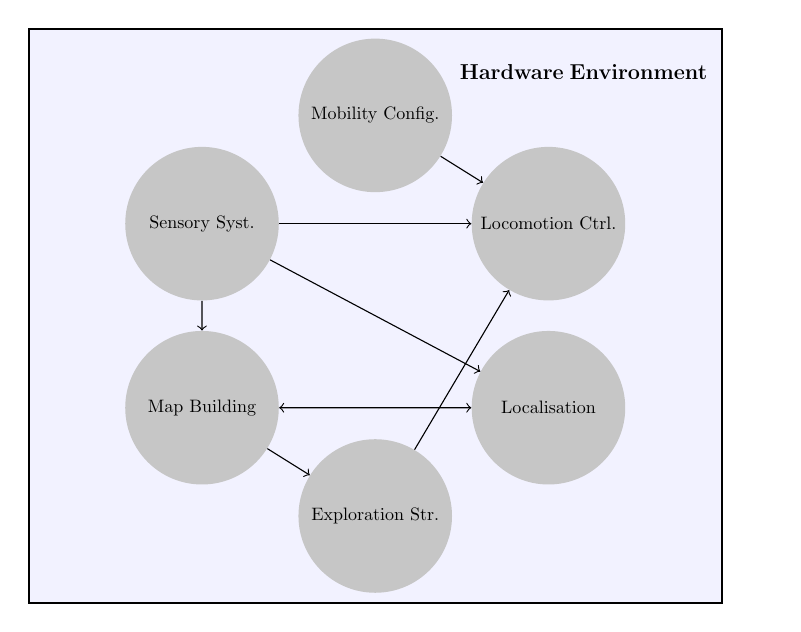
\begin{tikzpicture}[scale=0.55, every node/.style={scale=0.65}]
\draw[thick,fill=blue!5] (-8,2) rectangle (8,-11.25);
\draw (0,0) node (Mob) [circle,fill=gray!45,minimum size=3cm] {Mobility Config.};
\draw (-4,-2.5) node (Sense) [circle,fill=gray!45,minimum size=3cm] {Sensory Syst.};
\draw (4,-2.5) node (Loco) [circle,fill=gray!45,minimum size=3cm] {Locomotion Ctrl.};
\draw (-4,-6.75) node (Map) [circle,fill=gray!45,minimum size=3cm] {Map Building};
\draw (4,-6.75) node (Local) [circle,fill=gray!45,minimum size=3cm] {Localisation};
\draw (0,-9.25) node (Expl) [circle,fill=gray!45,minimum size=3cm] {Exploration Str.};

\draw[->] (Sense) -- (Local);
\draw[->] (Sense) -- (Map);
\draw[->] (Sense) -- (Loco);

\draw[->] (Map) -- (Expl);
\draw[<->] (Map) -- (Local);

\draw[->] (Mob) -- (Loco);

\draw[->] (Expl) -- (Loco);

\node[text width=6cm] at (5.5,1) 
    {\large \textbf{Hardware Environment}};

\end{tikzpicture}
\vspace{0.5cm}
\caption{The interdependencies of each of the six main subsystems, encapsulated by the hardware environment.}
\end{figure}

Each of the subsystems outlined above do not operate in isolation, rather, they have interdependencies. This means design considerations made in one subsystem have an impact on design considerations in other subsystems. Moreover, each of these subsystems operates in a hardware environment consisting of the robotic chassis, the computational hardware, and the power system. The set of interdependencies can be seen in Figure 1 - the hardware environment is pictured as the rectangle encapsulating .\\

A critical analysis consists of three main components: detailing how each of the competing choices for a design element work; analysing the advantages and disadvantages of each; and evaluating the best choice for the design task. This report is structured with six sections of the report which discuss competing design choices for each of the six subsystems outlined above. Each of these sections will culminate by looking at the advantages and disadvantages of each design choice. The next section of the report will briefly outline the design choices for the low complexity, moderate complexity, and high complexity designs. The final section of the report will evaluate each of the designs and provide a final recommendation on design choice.  

%-----------------------------------------------------
\section{Mobility Configuration}

Mobility configuration refers to the type of wheel used, and their geometrical arrangement on the chassis. This will affect manoeuvrability of the robot, and kinematic complexity governing the robot's movement. Typically, the more complex the kinematics, the more difficult it is to control the robot (Siegwart \& Nourbakhsh, 2004). The Pololu Dagu Rover 5 is the robot chassis specified by the client to be included in the final design, which is shown in Figure 2. The chassis has two principal configurations which are readily available:
\begin{itemize}
\item \textbf{Four motors, with Swedish 45 wheels:} each motor drives one of the 4 wheels directly (Swedish 45 wheels can be seen in Figure 3);
\item \textbf{Two motors, with tracked wheels:} each motor drives one of the two wheels directly, and the remaining two wheels are each driven by one of the robot tracks (see Figure 2)
\end{itemize}

\begin{figure}[h]
\centering
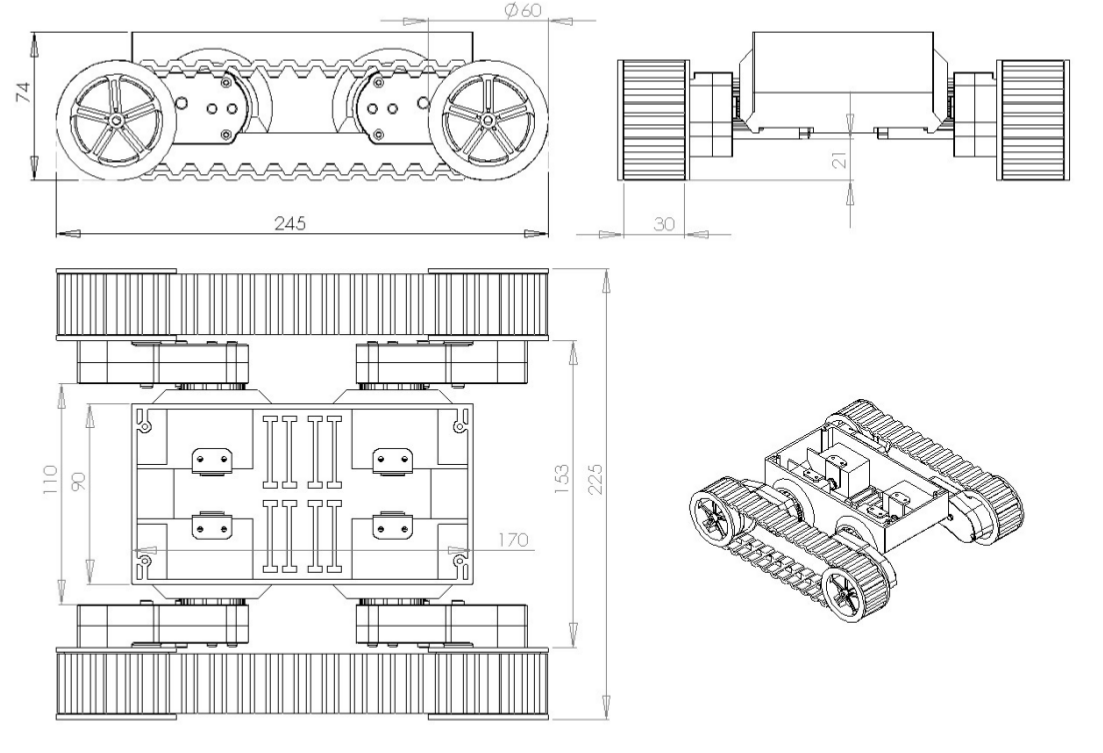
\includegraphics[scale=0.28]{fig1}
\caption{Detailed schematic of the Pololu Dagu Rover 5 chassis, set up with two motors and tracked wheels. (Source: Rover 5 Datasheet)}
\end{figure}

The design which uses four Swedish 45 wheels, shown in Figure 5, provides a high level of manoeuvrability. The design facilitates movement in any trajectory in the plane, however, this comes with increased kinematic complexity, making it more difficult to control. Tracked wheel design provides excellent robustness when dealing with significant floor discontinuity found in unstructured terrain. The design is a special implementation of a differential drive referred to as skid steering. The configuration intentionally relies on wheel slippage in order to make turns. This is problematic when relying on navigation schemes that utilise odometry for navigation (Borenstein, Everett, and Feng, 1996). A third configuration, which would require some chassis modification, can be seen in Figure 6. The configuration employs two motors, however, the tracks are removed from the chassis. Further, a passive spherical wheel (see Figure 4) would be mounted to the opposite end of the chassis. This configuration is widely used in AWR design, meaning that governing kinematics are simple and well documented, allowing for less complex control schemes. The main drawback to this design is no ready way to attach the spherical wheel to the chassis - a mount would have to be designed to allow for this. Table 1 provides a summary of the advantages and disadvantages for each of the three considered designs, and overall design evaluation can be found in Section 11.

\begin{figure}[h]
\centering
\begin{minipage}[t]{0.45\textwidth}
\centering
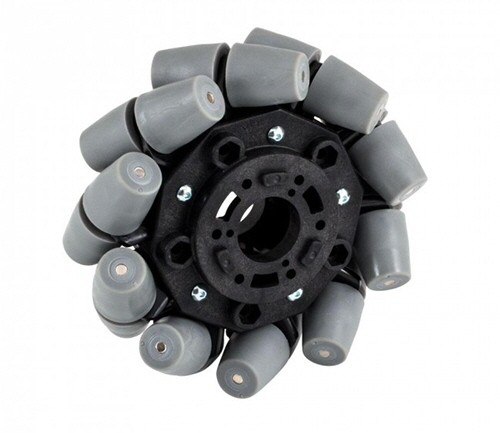
\includegraphics[scale=0.25]{omni_wheel}
\caption{Swedish 45 wheel, which has passive rollers around the wheel circumference, allowing movement along many different trajectories. (Source: \protect\url{http://www.core77.com})}
\end{minipage}
\hspace{1cm}
\begin{minipage}[t]{0.45\textwidth}
\centering
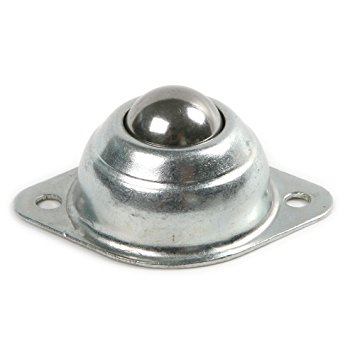
\includegraphics[scale=0.3]{ball_bearing}
\caption{Passive spherical wheel, providing omnidirectional movement. (Source: https://www.robotgear.com.au)}
\end{minipage}
\end{figure}
\begin{figure}[h]
\centering
\begin{minipage}[t]{0.45\textwidth}
\centering
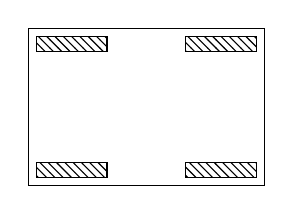
\begin{tikzpicture}
\draw (0,0) rectangle (3,2);
\draw[pattern=north west lines] (0.1,0.1) rectangle (1,0.3);
\draw[pattern=north west lines] (0.1,1.9) rectangle (1,1.7);
\draw[pattern=north west lines] (2.9,0.1) rectangle (2,0.3);
\draw[pattern=north west lines] (2.9,1.9) rectangle (2,1.7);
\end{tikzpicture}
\caption{The geometrical arrangement of the four omnidirectional wheels, each driven by a separate motor, allows the robot to move any trajectory in the plane.}
\end{minipage}
\hspace{1cm}
\begin{minipage}[t]{0.45\textwidth}
\centering
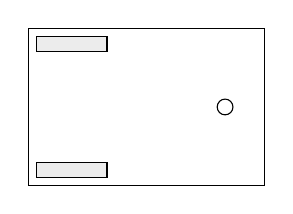
\begin{tikzpicture}
\draw (0,0) rectangle (3,2);
\draw[fill=gray!15] (0.1,0.1) rectangle (1,0.3);
\draw[fill=gray!15] (0.1,1.9) rectangle (1,1.7);
\draw (2.5,1) circle (0.1cm);
\end{tikzpicture}
\caption{The geometrical arrangement shows two standard wheels, each driven by a separate motor, in a differential drive configuration. A passive omnidirectional spherical wheel mounted at the opposite end of the chassis.}
\end{minipage}
\end{figure}

\begin{table}[h]
\centering 
\caption{Summary of the advantages and disadvantages of the design considerations for the mobility configuration}\footnotesize
\begin{tabular}{cp{4.7cm}p{0.1cm}p{4.7cm}p{0.1cm}p{4.7cm}}
\toprule
& \textbf{Four motors, with Swedish \newline 45 wheels} & & \textbf{Two motors, with tracked \newline wheels} & & \textbf{Differential Drive, with passive omnidirectinal wheel}\\
\midrule
\multirow{2}{*}[-0.35cm]{\rotatebox[origin=c]{90}{\textbf{Advantages}}} & \begin{itemize}[leftmargin=0.3cm] \item The design has increased manoeuvrability \item Inverse kinematics are similar to multi-dof robotic arm, since there are no non-holonomic constraints \end{itemize} & & \begin{itemize}[leftmargin=0.3cm] \item The design is already implemented on the Rover 5 chassis \item The dynamics are based on a simple differential drive model so is easy to understand \end{itemize} & & \begin{itemize}[leftmargin=0.3cm] \item The design is one of the most widely used and system dynamics are well documented \end{itemize} \\
\midrule
\multirow{2}{*}[-0.8cm]{\rotatebox[origin=c]{90}{\textbf{Disadvantages}}} & \begin{itemize}[leftmargin=0.3cm] \item The design requires more power to run the additional two motors \item Mathematical description of system dynamics is complicated and would be harder to understand \item Additional motors and enconders would need to be installed\end{itemize} & & \begin{itemize}[leftmargin=0.3cm] \item The design is based on a slippage model which is difficult to control \item Odometry errors from slippage require sophisticated localisation techniques like SLAM for correction \item Non-holonomic constraint means difficult to implement high level control \end{itemize} & & \begin{itemize}[leftmargin=0.3cm] \item Passive omnidirectional wheel has no readily available mounting \item Non-holonomic constraint means difficult to implement high level control \end{itemize} \\
\bottomrule
\end{tabular}
\end{table}

\clearpage

%-------------------------------------------------------------
\section{Sensory System}
The sensory system of a robot provides facility to capture data about the robot itself, and the robot's environment. This data is used to build maps, determine the robot's position (relative localisation), or control locomotion along some planned path - tasks which are of interest in the design of an AWR. Siegwart \& Nourbakhsh (2004) classify sensors into two types: Proprioceptive, or Exteroceptive. Both sensor types will be important for design considerations.
\subsection{Proprioceptive Sensors}
Proprioceptive sensors are those sensors which provide internal information about the robot. Examples of this type of information are robot velocity, acceleration, wheel rotation, or the robot's heading (Leung, 2003). These types of sensors are typically used to estimate the change in robot position over time, sometimes referred to as relative localisation (Ippoliti, Jetto, \& Longhi, 2005). There are two widely accepted ways of approaching this:
\begin{enumerate}
\item \textbf{Odometry:} uses encoders to measure wheel rotation, which is in turn used to evaluate relative position, heading, and vehicle velocity (Everett, 1995);
\item \textbf{Inertial Navigation:} uses accelerometers, together with gyroscopes, to yield position, velocity, acceleration, and heading (Borenstein, Everett, \& Feng, 1995)
\end{enumerate}

These types of sensors are also important for low level locomotion control. This subsection of the report will consider two types of Proprioceptive Sensors which could be used: optical encoders, and inertial measurement units.

\subsubsection{Incremental Optical Rotary Encoders}
Incremental optical rotary encoders are devices which will measure the angular velocity and infer relative position of some shaft, or one of the gears in a gear train. A black and white patterned disk, like the one shown in Figure 7, is attached to the shaft of interest. More segments implies higher encoder resolution. Infrared (IR) light is emitted onto the disk, and the reflected IR is detected with a sensor. IR light is reflected from lighter panels, and absorbed by darker panels. When the patterned wheel spins with the shaft of interest, the IR detector receives alternating high and low signals (Borenstein, Everett, and Feng, 1996).\\

\begin{figure}[h]
\centering
\begin{minipage}[t]{0.45\textwidth}
\centering
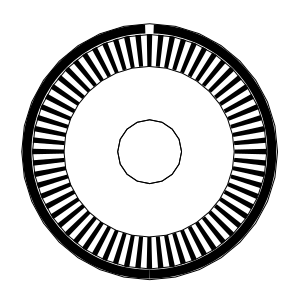
\includegraphics[height=4.4cm]{optical_enc}
\caption{Black and white patterned disk on an optical encoder. White sections reflect IR light, and black absorb IR light. (Source: Siegwart, \& Nourbakhsh, 2004)}
\end{minipage}
\hspace{1cm}
\begin{minipage}[t]{0.45\textwidth}
\centering
\frame{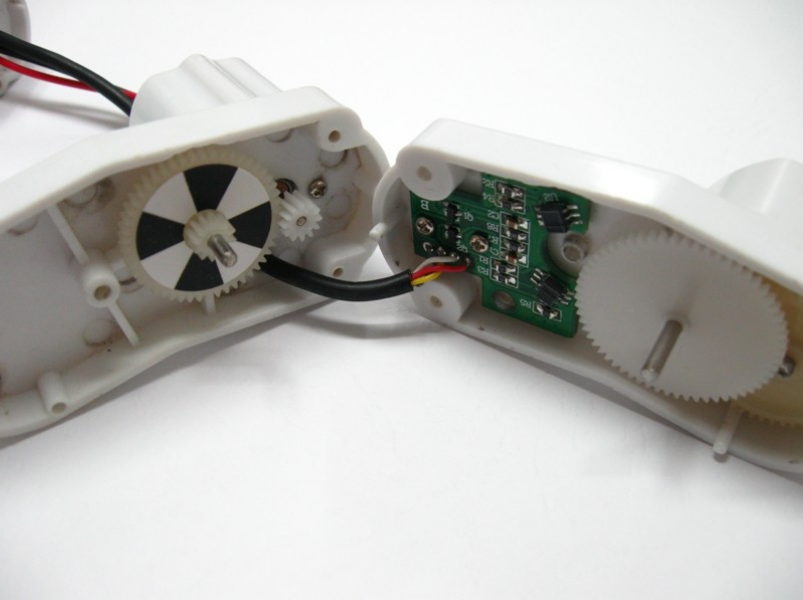
\includegraphics[height=3.9cm]{optical_encoder_actual}}
\caption{An incremental quadrature optical rotary encoder is provided on each of the two motors that come with the Rover 5 chassis. (Source: Rover 5 Datasheet)}
\end{minipage}
\end{figure}

A single IR detection sensor is unable to indicate the direction in which the shaft is spinning. Quadrature rotary encoders, shown in Figure 9, make use of two IR sensors. The sensor pair are mounted 90$^o$ out of phase with each other. Spinning the encoder creates two high/low signal patterns which are 90$^o$ out of phase, as shown in Figure 10. If the shaft is spinning in one direction the state sequence is $S_1 S_2 S_3 S_4$, and the sequence is reversed if the shaft is spinning in the opposite direction. There are two Quadrature encoders equipped to the motors on the Rover 5 chassis, like the one shown in Figure 8. The resolution, which is measured in counts per revolution (CPR), tells us how many pulse transitions to expect for one given wheel revolution. The encoders on the Rover 5 chassis undergo 1000 pulse transitions every 3 revolutions - the encoders are aptly named 333 CPR. This information can be used to calculate the distance travelled by a wheel for 1 pulse count. If the Rover 5 chassis has wheels equipped of $R$ millimeters in diameter, then the distance travelled for a single revolution is the wheel circumference:
\begin{align*}
C 	= 2 \cdot \pi \cdot radius = \pi \cdot R = 1 \ \ \texttt{rev}
\end{align*}

Hence, if there are 1000 pulse transitions for 3 revolutions implies that the angular displace for a single pulse, $\beta_{pulse}$, is given by:
\begin{align}
1000 \times \beta_{pulse} &= 3 \ \ [\texttt{rev}] \nonumber\\
\beta_{pulse} &= \frac{3 \ \ [\texttt{rev}]}{1000} \times \frac{2 \cdot \pi \ \ {[\si{\radian}}]}{1 \ \ [\texttt{rev}]} \nonumber\\
\beta_{pulse} &= \frac{6 \cdot \pi}{1000} \ \ [\si{\radian}]
\end{align}

Assuming we have some sampling period, $\Delta T$, and the pulse count is specified as $N_K$ for discrete time $k$, then using equation (1) we can arrive at an estimate for angular velocity:
\begin{align}
\omega_k = \frac{(N_{k} - N_{k-1}) \cdot 6 \cdot \pi}{1000} \ \ [\si{\radian\per\sec}]
\end{align}


\begin{figure}[h]
\centering
\begin{minipage}{0.45\textwidth}
\centering
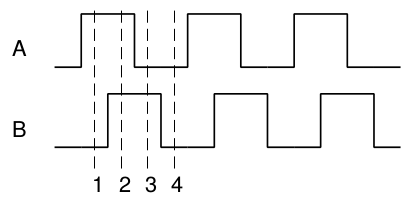
\includegraphics[scale=0.4]{optical_encoder_signal}
\caption{The two idealised signals generated by the IR sensor pair on a Quadrature Encoder. The two waves are 90$^o$ out of phase. (Source: Siegwart, \& Nourbakhsh, 2004)}
\end{minipage}
\hspace{1cm}
\begin{minipage}{0.45\textwidth}
\centering
\captionof{table}{Four unique states from the two signals can be observed - the positions of these states are shown in Figure 10.}
\begin{tabular}{lll}
\toprule
\textbf{State} & \textbf{Ch A} & \textbf{Ch B}\\
\midrule
$S_1$ & HIGH & LOW\\
$S_2$ & HIGH & HIGH\\
$S_3$ & LOW & HIGH\\
$S_4$ & LOW & LOW\\
\bottomrule
\end{tabular}
\end{minipage}
\end{figure}

\begin{figure}[h]
\begin{minipage}{0.45\textwidth}
A simple example of how \textit{odometry} works can be seen by analysing straight-line motion, where the angular velocity of the wheels are equal: $\omega_{LW} = \omega_{RW}$. Consider Figure 7, where $X_{I}[k]$, and $Y_{I}[k]$ refer to the robots position in the global environment at some instant $n$, and the robot's current heading is given by $\theta$. Suppose the robot travels at some linear velocity, $(R \omega_k)$, over the discrete time period $\Delta T = t_{k} - t_{k-1}$. Note that $R$ is the wheel radius of the robot, and the angular velocity is measured by the rotary encoder. The global position of the robot at time $t_k$ is given by:
\begin{align*}
X_{I}[k] &= X_{I}[k-1] + (R \omega_k)\cdot \Delta T \cdot \sin \theta\\
Y_{I}[k] &= Y_{I}[k-1] + (R \omega_k) \cdot \Delta T \cdot \cos \theta
\end{align*}
\vspace{0.5cm}
\end{minipage}
\hspace{1.25cm}
\begin{minipage}{0.45\textwidth}
\centering
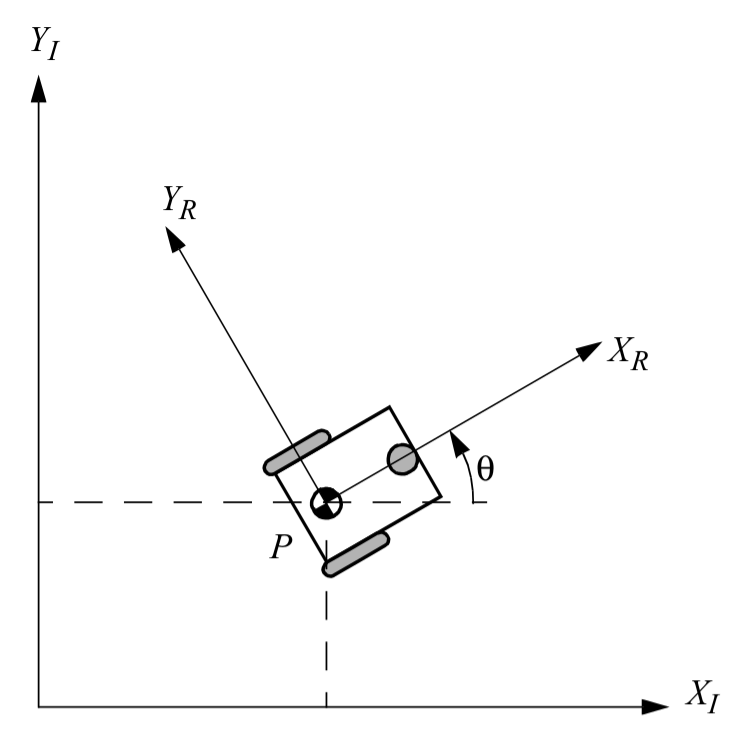
\includegraphics[scale=0.2]{odometry}
\caption{The robot in the global coordinate frame denoted by the subscript $I$. The coordinate frame attached to the robot is denoted with a subscript $R$, and allows us to define the robot heading, $\theta$. (Source: Siegwart, \& Nourbakhsh, 2004)}
\end{minipage}
\end{figure}

Table 3 provides a summary of the advantages and disadvantages of using an optical rotary encoder to calculate odometry.

\begin{table}[h]
\centering
\caption{Summary of the advantages and disadvantages of using optical rotary encoders to calculate odometry} \footnotesize
\begin{tabular}{p{8cm}p{8cm}}
\toprule
\textbf{Advantages} & \textbf{Disadvantages}\\
\midrule
\begin{itemize}[leftmargin=0.3cm] \item Two quadrature optical encoders come pre-installed with the Rover 5 chassis specified by the client \item Easy to understand, and straightforward to implement \item The quick brown fox jumped over the lazy dog \end{itemize} & \begin{itemize}[leftmargin=0.3cm] \item There are errors present in the measurements provided by encoders given the discrete nature of their pulses \item Odometry position is based on a cumulative method, meaning that over time errors grow without bound \item Odometry error is particularly sensitive to changes in robot orientation \end{itemize}\\
\bottomrule
\end{tabular}
\end{table}

\newpage
\subsubsection{Accelerometer \& Gyroscopes (IMU)}
Accelerometers are used to measure external forces acting on the vehicle, which can be used to determine dynamic accelerations (Borenstein, Everett, \& Feng, 1996). It must be noted that the sensor cannot distinguish between static gravitational force, and dynamic forces - this means care is required when interpreting sensor results. The on-board accelerometer provided with the myRIO utilises a microelectromechanical system (MEMS). The device has two terminals, with finger like arrangement acting as tiny capacitance plates, as shown in Figure 11. One of the terminals has mass attached to it, and when the accelerometer is moved along the axis of interest, the plates move, which changes the capacitance. Measured change in capacitance provides an estimate of the acceleration. Note that there are actually three accelerometers in the myRIO device, each one mounted on a different mutually orthogonal axis.\\

Gyroscopes are used to measure changes in the vehicle orientation. A MEMS gyroscopic sensor has a mass which oscillates at some velocity. When an angular velocity is applied to the sensor, the mass experiences a force due to the Coriolis effect. Similarly to the MEMS accelerometer, the MEMS gyroscope makes use of tiny capacitance plates. It is the change in capacitance that allows the estimation of the applied angular velocity (Dudek, \& Jenkins, 2008). A single axis MEMS gyroscope can be seen in Figure 12. Typically, a MEMS gyroscopic sensor has three gyroscopes mounted on mutually orthogonal axes. 
\begin{figure}[h]
\hspace{0.5cm}
\begin{minipage}[t]{0.40\textwidth}
\centering
\frame{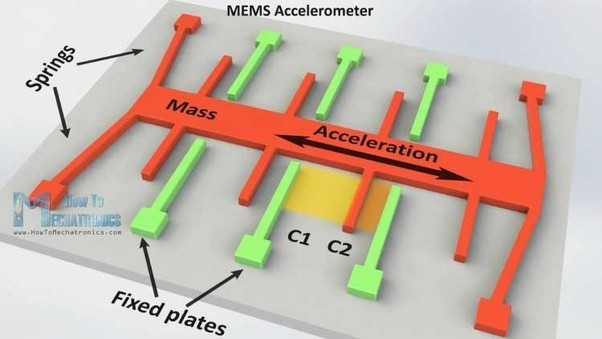
\includegraphics[height=5cm]{mems_accelerometer}}
\caption{MEMS accelerometer. As the mass moves due to acceleration, the plates come closer together, or further apart, causing a measurable change in capacitance. (Source: \protect\url{https://www.sensorsmag.com})}
\end{minipage}
\hspace{3cm}
\begin{minipage}[t]{0.3\textwidth}
\centering
\frame{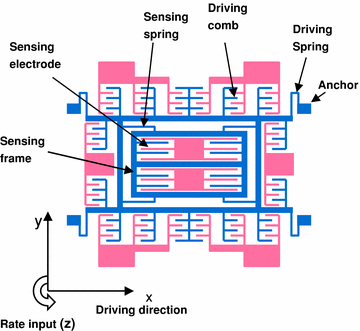
\includegraphics[height=5cm]{mems_gyroscope}}
\caption{MEMS gyroscope. the plates come closer together, or further apart, causing a measurable change in capacitance. (Source: \protect\url{http://iopscience.iop.org})}
\end{minipage}
\end{figure}

An accelerometer and gyroscope used in conjunction is often referred to as an Inertial Measurement Unit (IMU). An IMU can be employed to determine relative localisation of an AWR - the process can be seen in Figure 13 (Dudek, \& Jenkins, 2008). In this instance, the robot is constrained to movement in the $x$-$y$ plane, so we position the $z$-axis of the gyroscope orthogonal to this plane in order to detect rotational velocities about the $z$-axis. These rotational velocities are integrated and added to the initial heading to determine the robot's heading with respect to the Global frame. The $x$ and $y$ axes of the accelerometer are fixed on the robot and aligned with $X_R$ and $Y_R$, respectively (as shown in Figure 10). Detected accelerations in either the $x$ or $y$ axes can be integrated once to determine the relative velocity, or twice to determine the relative position. Combining these with the initial conditions allows the determination of the global velocity, and position. According to Dudek \& Jenkins (2008) using accelerometers for inertial navigation is prone to error since the sensor measurements are integrated twice. Table 4 summarises the advantages and disadvantages of using accelerometers and gyroscopes for inertial navigation.

\begin{figure}[h]
\centering
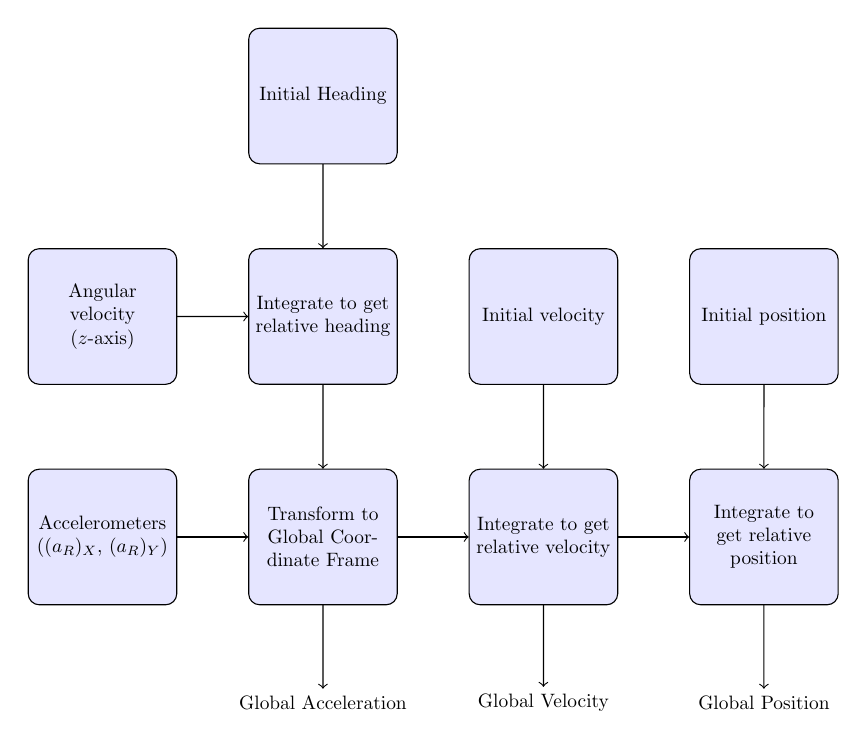
\begin{tikzpicture}[
block/.style={rectangle, draw, minimum width=7em,
text centered, rounded corners, minimum height=7em, text width=7em, fill=blue!10, node distance=4cm},
scale=0.7, every node/.style={scale=0.7}
]
\node[block] (n1) {Accelerometers ($(a_R)_X$, $(a_R)_Y$)};
\node[block, right of=n1] (n2) {Transform to Global Coordinate Frame};
\node[block, right of=n2] (n3) {Integrate to get relative velocity};
\node[block, right of=n3] (n4) {Integrate to get relative position};
\node[block, above of=n3] (n5) {Initial velocity};
\node[block, above of=n4] (n6) {Initial position};
\node[block, above of=n1] (n7) {Angular velocity ($z$-axis)};
\node[block, right of=n7] (n8) {Integrate to get relative heading};
\node[below of=n2, node distance=3cm] (n9) {Global Acceleration};
\node[below of=n3, node distance=3cm] (n10) {Global Velocity};
\node[below of=n4, node distance=3cm] (n11) {Global Position};
\node[block, above of= n8] (n12) {Initial Heading};


\draw[->] (n1)--(n2);
\draw[->] (n2)--(n3);
\draw[->] (n3)--(n4);
\draw[->] (n5)--(n3);
\draw[->] (n6)--(n4);
\draw[->] (n7)--(n8);
\draw[->] (n8)--(n2);
\draw[->] (n2)--(n9);
\draw[->] (n3)--(n10);
\draw[->] (n4)--(n11);
\draw[->] (n12)--(n8);
\end{tikzpicture}
\caption{Computational flow diagram used for determining the global heading, acceleration, velocity, and position using inertial navigation.}
\end{figure}

\begin{table}[h]
\centering
\caption{Summary of the advantages and disadvantages of using an IMU for inertial navigation} \footnotesize
\begin{tabular}{p{8cm}p{8cm}}
\toprule
\textbf{Advantages} & \textbf{Disadvantages}\\
\midrule
\begin{itemize}[leftmargin=0.3cm] \item The myRIO has a built in accelerometer \item The sampling frequency is higher compared to optical encoders \end{itemize} & \begin{itemize}[leftmargin=0.3cm] \item Integrating the reported acceleration from the sensors means that this type of navigation is sensitive to errors \item Typically, due to propensity for error, these systems are used concurrently with absolute localisation such as SLAM, which is technically challenging to implement \end{itemize}\\
\bottomrule
\end{tabular}
\end{table}

\newpage

\subsection{Exteroceptive Sensors}
Exteroceptive sensors are those sensors which acquire information from the robot's environment (Leung, 2003). Examples of this type of information include distance measurements, light intensity, and sound amplitude. The two main applications of these sensors for AWRs are map generation, and absolute localisation. The remainder of this subsection will take a closer look at the advantages and disadvantages of three of these sensors: infrared distance, time of flight ultrasonic, and an RBGD camera.

\subsubsection{Infrared Distance Sensor}
The basic operating principle of the IR sensors is based on infrared light. By looking at where the light hits the detector, it is possible to calculate the angle of the light and from that angle, derive the distance to the object. Figures 14 and 15 illustrates the basic operating principle of the ranging technique.
\begin{figure}[h]
\centering
\begin{minipage}[t]{0.45\textwidth}
\centering
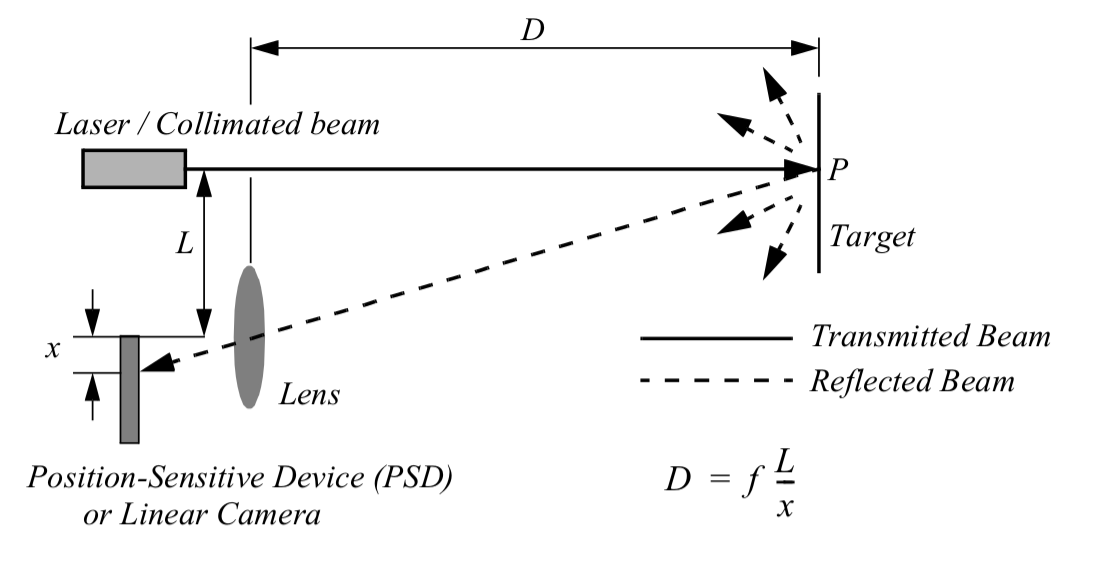
\includegraphics[scale=0.25]{1d_IR_triang}
\caption{The 1D IR ranging sensor sends IR light which reflects from the target surface, entering the IR sensor lens at some angle. Triangulation is used to determine the distance to the target. (Source: Siegwart \& Nourbakhsh, 2004)}
\end{minipage}
\hspace{1cm}
\begin{minipage}[t]{0.45\textwidth}
\centering
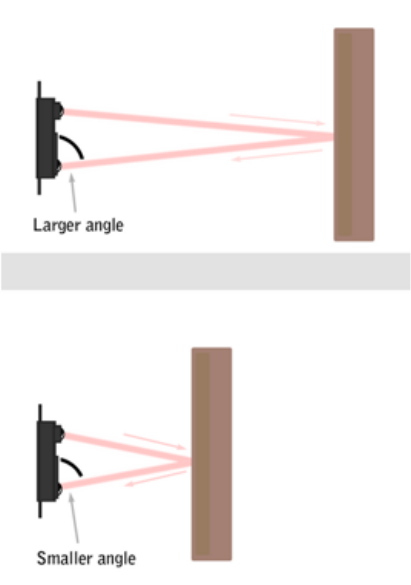
\includegraphics[scale=0.25]{1d_IR_example}
\caption{An example showing how the angle of reflected IR light varies on the IR sensor array for different target distances.}
\end{minipage}
\end{figure}

Two different 1D IR ranging sensors were selected, based on their different ranging properties. The SHARP GP2YD120 has an accurate measurement range of 40 millimetres to 300 millimetres, and the SHARP GP2Y0A21YK0F has an accurate measurement range of 100 millimetres to 800 millimetres. The SHARP GP2Y0A21YK0F sensor can be seen in Figure 16. In both SHARP IR sensors the dependence between voltage output and corresponding distance is not linear, as shown in the Figures 16 and 17 below. There are 2 approaches to calibrating a sensor model for use on a mobile robotics platform. One way is to focus on a linear region of operation, and determine a simple linear model using regression techniques. This linearised model can then be implemented programatically, however, the result will carry some error since the linear model is only an approximation for the non-linear behaviour of the sensor. Another method simply relies on extracting voltage and distance values at a reasonably high resolution, and programatically implementing these as a discrete lookup table. This allows the sensor to be used over a broader range of operation, but also carries error given the discrete nature of measurements. Table 7 summarises the advantages and disadvantages of this sensor.
\vspace{-2cm}
\begin{figure}
\centering
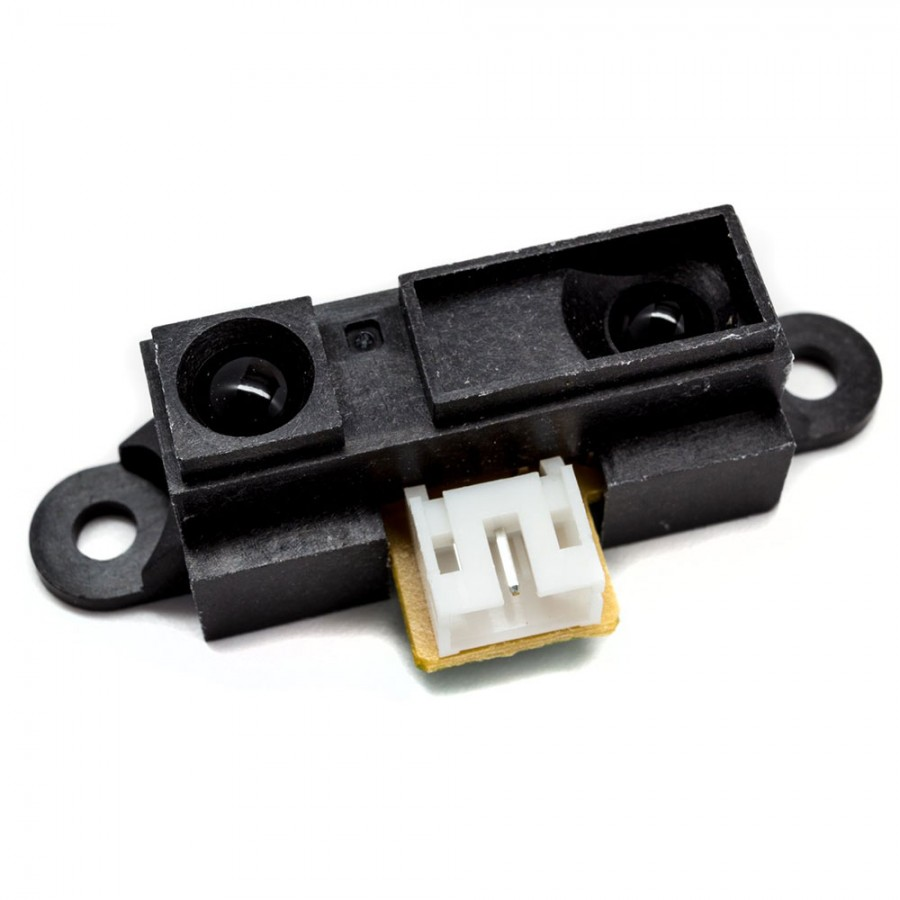
\includegraphics[scale=0.08]{sharp_sensor}
\caption{A picture of the SHARP GP2YD120 sensor.}
\end{figure}

\begin{figure}[h]
\centering
\begin{minipage}[c]{0.45\textwidth}
\centering
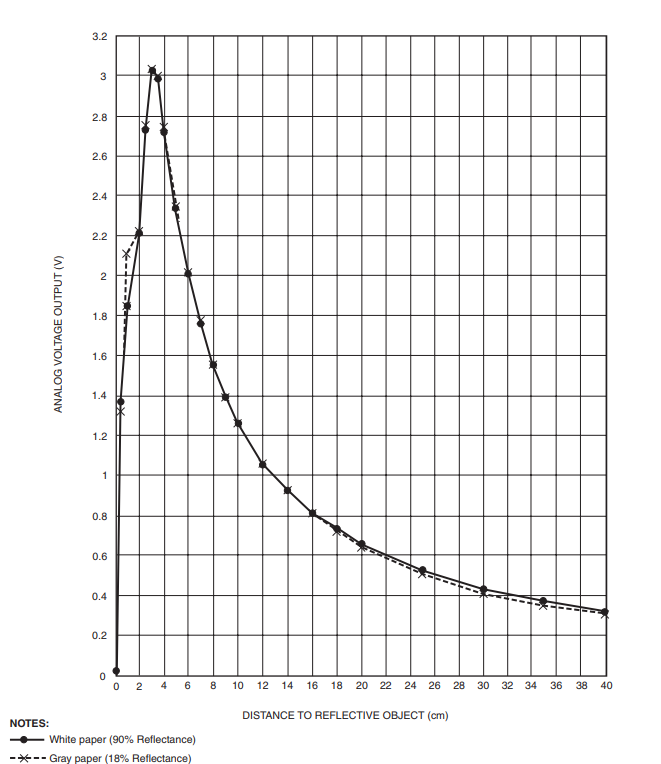
\includegraphics[scale=0.4]{GP2Y_short}
\caption{Voltage and ranged distance profile for the SHARP GP2YD120 sensor. (Source: SHARP GP2YD120 Datasheet)}
\end{minipage}
\hspace{1cm}
\begin{minipage}[c]{0.45\textwidth}
\centering
\captionof{table}{Values corresponding to the voltage and ranged distance profile for the SHARP GP2YD120 sensor.}
\begin{tabular}{cc}
\toprule
\textbf{Voltage Output ($\si{\volt}$)} & \textbf{Distance ($\si{\centi\meter}$)}\\
\midrule
3 & 3.5\\
2.8 & 4\\
1.6 & 8\\
1.1 & 12\\
0.85 & 16\\
0.7 & 20\\
0.6 & 24\\
0.5 & 28\\
0.4 & 32\\
0.35 & 36\\
0.3 & 40\\
\bottomrule
\end{tabular}
\end{minipage}
\end{figure}

\begin{figure}[h]
\centering
\begin{minipage}[c]{0.45\textwidth}
\centering
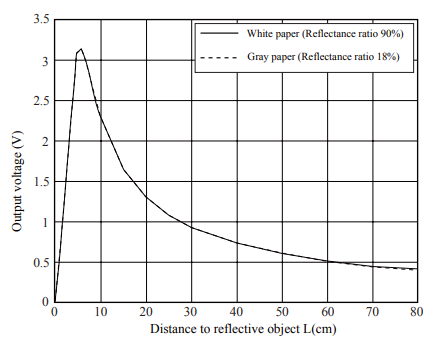
\includegraphics[scale=0.5]{GP2Y_long}
\caption{Voltage and ranged distance profile for the SHARP GP2Y0A21YK0F sensor. (Source: SHARP GP2Y0A21YK0F Datasheet)}
\end{minipage}
\hspace{1cm}
\begin{minipage}{0.45\textwidth}
\centering
\captionof{table}{Values corresponding to the voltage and ranged distance profile for the SHARP GP2Y0A21YK0F sensor.}
\begin{tabular}[c]{cc}
\toprule
\textbf{Voltage Output ($\si{\volt}$)} & \textbf{Distance ($\si{\centi\meter}$)}\\
\midrule
3.1 & 5\\
3.2 & 6\\
3 & 7\\
2.7 & 8\\
2.3 & 10\\
1.6 & 15\\
1.25 & 20\\
1.1 & 25\\
0.8 & 30\\
0.75 & 40\\
0.6 & 50\\
0.4 & 80\\
\bottomrule
\end{tabular}
\end{minipage}
\end{figure}

\clearpage

\begin{table}
\centering
\caption{Summary of the advantages and disadvantages of the 1D IR ranging sensors} \footnotesize
\begin{tabular}{p{8cm}p{8cm}}
\toprule
\textbf{Advantages} & \textbf{Disadvantages}\\
\midrule
\begin{itemize}[leftmargin=0.3cm] \item Low cost \item Low power \item Reasonable accuracy for close objects \end{itemize} & \begin{itemize}[leftmargin=0.3cm] \item Poor accuracy for objects at a distance - limited by geometry \end{itemize}\\
\bottomrule
\end{tabular}
\end{table}

\subsubsection{Ultrasonic Time of Flight Sensor}
Like the 1D IR ranging sensors, an ultrasonic sensor provides distance measurement. The basic operating principle is illustrated in the Figure 19. It works by transmitting an
ultrasonic (well above human hearing range) burst and providing an output pulse that corresponds to the time required for the burst echo to return to the sensor. By measuring the echo pulse width, the distance to target can easily be calculated.

\begin{figure}[h]
\centering
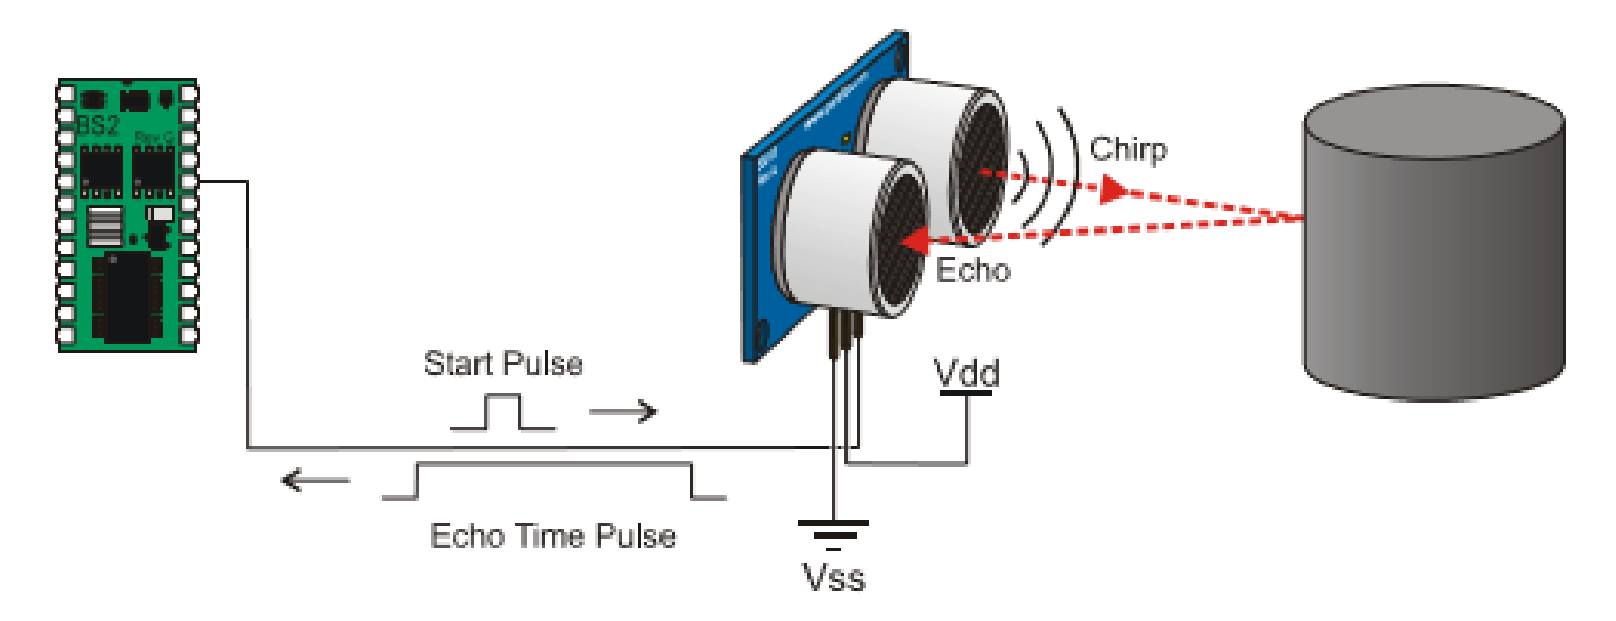
\includegraphics[scale=0.2]{ultrasonic_tof}
\caption{Typically an ultrasonic sensor will emit a sonic burst and trigger an ECHO pulse. The ECHO pulse is triggered again when the sonic burst returns to the sensor. The time duration of the ECHO pulse is used to measure the distance to the target.}
\end{figure}

The distance can be calculated by multiplying the speed of sound, $\nu$, by the total time of travel, $\Delta t$. Distance to target, $L$, can be determined as follows:
\begin{align*}
L = \frac{\Delta t \cdot \nu}{2} [\si{\centi\meter}]
\end{align*}

Note that the 2 in the denominator represents the fact that ultrasonic wave crosses over the unknown distance twice. Noting that the speed of sound is 343 $\si{\meter\per\second}$ at 20$\si{\celsius}$. Hence,
\begin{align*}
L = \frac{\Delta t \cdot 343}{2} = 171.5 \times \Delta t \ \  [\si{\meter\per\second}]
\end{align*}

Principal factors affecting the range ability are ambietn temperature, $T_C$. The speed of sound is very sensitive to variations in temperature, hence it is important to calibrate the sensor in a similar temperature to the operating environment. The equation below describes the sensitivity level of the sensor in response to the temperature variations:
\begin{align*}
\Delta \nu = 331.5 + (0.6 \times T_C)
\end{align*}

The advantages and disadvantages of this sensor are summarised in Table 8.
\begin{table}[h]
\centering
\caption{Summary of the advantages and disadvantages of the ultrasonic time of flight sensor} \footnotesize
\begin{tabular}{p{8cm}p{8cm}}
\toprule
\textbf{Advantages} & \textbf{Disadvantages}\\
\midrule
\begin{itemize}[leftmargin=0.3cm] \item Simple to implement \item Low power \item Reasonably accurate over a range of distances \end{itemize} & \begin{itemize}[leftmargin=0.3cm] \item Accuracy of the sensor is based on the acoustic reflective properties of the target \item Sensor can give incorrect reading due to cross talk from other sensors, or reflected acoustic waves \item Targets with non-orthogonal surfaces may produce errors \end{itemize}\\
\bottomrule
\end{tabular}
\end{table}

\newpage

\subsubsection{RGBD Sensor}
An RGBD sensor captures a 2D pixel array on red, green, and blue channels using a monocular camera. Further, the sensor captures depth information by measuring the deformation of reflections from structured infra-red (IR) light emitted into the environment (Ganganath, \& Leung, 2012). The Microsoft Kinect, shown in Figure 20, is a low cost RGBD camera which is readily employed in robotics projects requiring high fidelity environmental information.
\begin{figure}[h]
\centering
\begin{minipage}{0.45\textwidth}
\centering
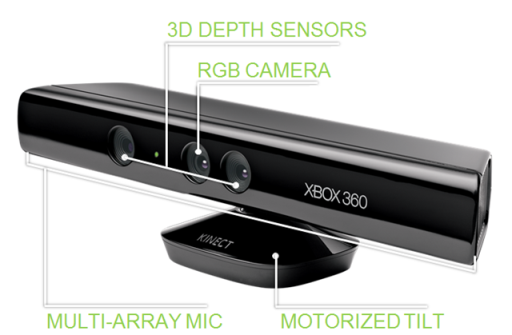
\includegraphics[scale=0.6]{kinect}
\caption{The Microsoft Kinect sensor, which comes with an optical RGB camera, IR structured light emitter, and IR sensor. The sensor combination can be used to create 3D point clouds of 640 $\times$ 480 resolution, with 11-bit depth resolution.}
\end{minipage}
\hspace{1cm}
\begin{minipage}{0.45\textwidth}
\centering
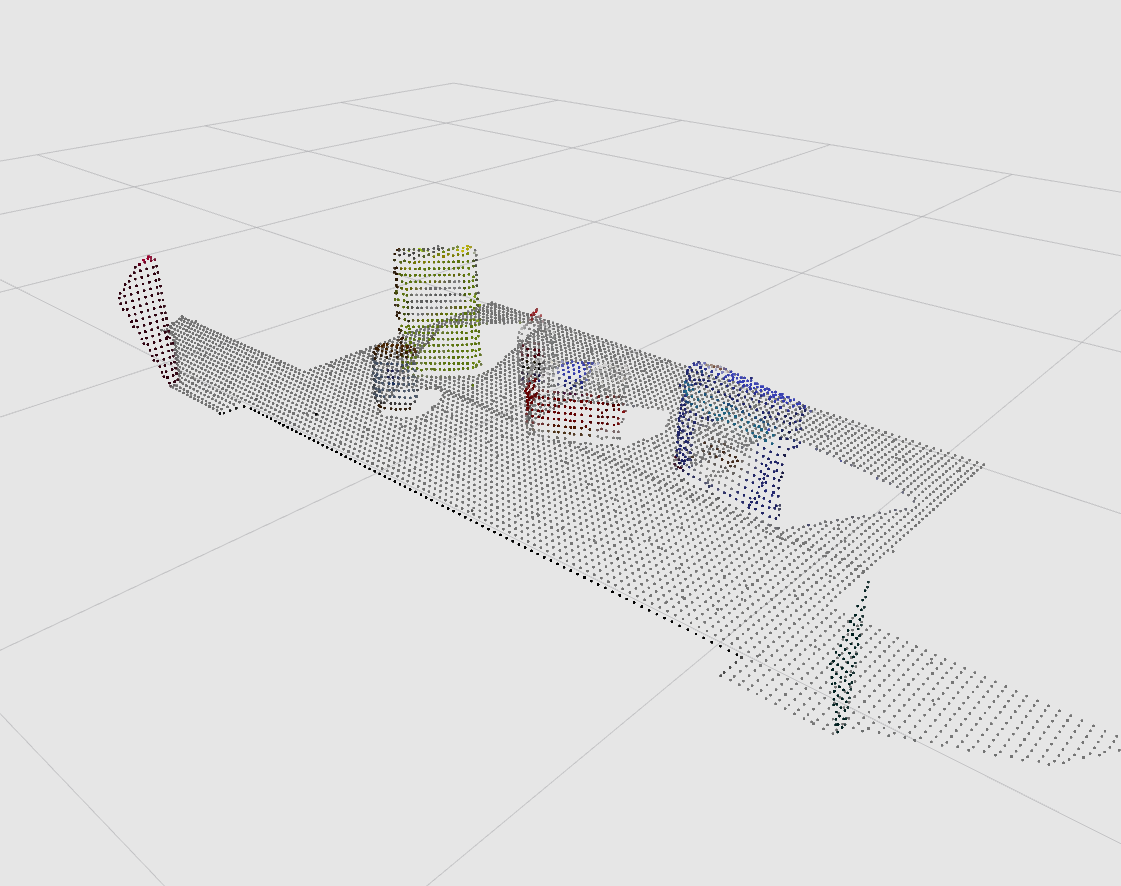
\includegraphics[scale=0.25]{kinect_voxel_ds}
\caption{Sensor data taken from a Microsoft Kinect and used to create a 3D point cloud using the $\texttt{pcl}$ library. The signal noise was removed using a statistical outlier filter, and the number of points in the point cloud reduced using Voxel downsampling. Image taken from Reynolds (2018).}
\end{minipage}
\end{figure}

The Kinect depth sensor, and optical sensor, operate at a resolution of 640 $\times$ 480 pixels. Combining the optical RGB and IR depth information, allows the development of a point cloud consisting of approximately 300000 points (Kamarudin, Mamduh, Shakaff, \& Zakaria, 2014). Typically, some of the points are removed to reduce the amount required computational resources needed to process a point cloud. This is done using a process called Voxel downsamping. An example of a downsampled point cloud, generated from Kinect sensor data, can be seen in Figure 21. Point cloud representations of environments are desirable as they allow for the a number of sophisticated solutions to difficult problems associated with designing an AWR:
\begin{itemize}
\item The most notable of these solutions is SLAM, discussed in Section 6, which provides a way to correct odometry errors.
\item The other notable advantage of the Kinect is using the optical camera with a colour segmentation filter to detect the exit panel - this is discussed further in Section 9.3.2.  
\end{itemize}

Table 9 provides a summary of the advantages and disadvantages of using an RGBD camera, or not. 

\begin{table}[h]
\centering
\caption{Summary of the advantages and disadvantages of Kinect sensor} \footnotesize
\begin{tabular}{p{7.5cm}p{0.1cm}p{7.5cm}}
\toprule
\textbf{Advantages} & & \textbf{Disadvantages}\\
\midrule
\begin{itemize}[leftmargin=0.3cm] \item Sensor provides access to 3D point cloud which can be used for advanced computational schemes such as SLAM \item Optical RGB sensor could be utilised to detect the red exit panel using an Hue, Saturation, Value (HSV) image segmentation filter \end{itemize} & & \begin{itemize}[leftmargin=0.3cm] \item Technically challenging to implement many of the computational schemes that take advantage of the sensor \item Since AWR navigation is in 2D, additional information from 3D point clouds are not fully utilised \item Sensor is expensive \item Sensor requires a 12 $\si{\volt}$ power supply\end{itemize}\\
\bottomrule
\end{tabular}
\end{table}

\newpage

\section{Locomotion Control}
Locomotion, according to the Concise Oxford Dictionary, is the motion from place to place. In the context of a mobile robot, locomotion is the process by which the robot moves. This requires an application of force (Dudek, \& Jenkin, 2010), which in this instance is provided by two DC brushed motors, driving 86.8:1 gearboxes. The motors come pre-equipped with the Rover 5 chassis - the full motor specifications can be found in Table 1. 

\begin{figure}[h]
\begin{minipage}{0.45\textwidth}
Locomotion control is an important design consideration when building a mobile robot. The problem can be divided up into two categories: Low Level Control, and High Level Control. This section of the report discusses the design options for low level control strategies, and then provides some background information for high level control strategies.
\vspace{0.4cm}
\end{minipage}
\hspace{1cm}
\begin{minipage}{0.45\textwidth}
\centering
\caption{Specifications of the motors which come equipped with the Rover 5 chassis}
\footnotesize\begin{tabular}{lr}
\toprule
\textbf{Characteristic} & \textbf{Description}\\
\midrule
Voltage & 7.2 $\si{\volt}$\\
Unloaded Current & 210 $\si{\milli\ampere}$\\
Stall Current & 2.4 $\si{\ampere}$\\
Max Speed & 25 $\si{\centi\meter\per\second}$\\
\bottomrule
\end{tabular}
\end{minipage}
\end{figure}

\subsection{Low Level Control}
Low level control strategies are concerned with controlling the actual output of the motors - angular velocity (or angular position). The simplest way of accomplishing this is using open loop control. The basic control structure can be seen in Figure 23. Basically, the desired reference value, $r$, is fed to the controller, which send a control signal, $u$, to the   Open loop control systems are those in which actual system output has no effect on the control action (Ogata, 2010). The advantages of this type of control are that it is simple to implement with software.  

\tikzstyle{block} = [draw, fill=blue!20, rectangle, 
    minimum height=3em, minimum width=6em]
\tikzstyle{sum} = [draw, fill=blue!20, circle, node distance=1cm]
\tikzstyle{input} = [coordinate]
\tikzstyle{output} = [coordinate]
\tikzstyle{pinstyle} = [pin edge={to-,thin,black}]

\begin{figure}[h]
\centering
\begin{minipage}[t]{0.45\textwidth}
\centering
% The block diagram code is probably more verbose than necessary
\begin{tikzpicture}[auto, node distance=2cm,>=latex']
    % We start by placing the blocks
    \node [input, name=input] {};
    \node [block, right of=input] (controller) {Controller};
    \node [block, right of=controller, pin={[pinstyle]above:Disturbances},
            node distance=3cm] (system) {System};
    % We draw an edge between the controller and system block to 
    % calculate the coordinate u. We need it to place the measurement block. 
    \draw [->] (controller) -- node[name=u] {$u$} (system);
    \node [output, right of=system] (output) {};

    % Once the nodes are placed, connecting them is easy. 
    \draw [draw,->] (input) -- node {$r$} (controller);
    \draw [->] (system) -- node [name=y] {$y$}(output);
\end{tikzpicture}
\caption{Open loop control structure sees a reference signal, $r$, sent to the controller, which sends a control signal, $u$, to the system in order to control the desired output, $y$. The output does not need to be measured by sensors in this instance.}
\end{minipage}
\hspace{1cm}
\begin{minipage}[t]{0.45\textwidth}
\centering
% The block diagram code is probably more verbose than necessary
\begin{tikzpicture}[auto, node distance=2cm,>=latex']
    % We start by placing the blocks
    \node [input, name=input] {};
    \node [sum, right of=input] (sum) {};
    \node [block, right of=sum] (controller) {Controller};
    \node [block, right of=controller, pin={[pinstyle]above:Disturbances},
            node distance=3cm] (system) {System};
    % We draw an edge between the controller and system block to 
    % calculate the coordinate u. We need it to place the measurement block. 
    \draw [->] (controller) -- node[name=u] {$u$} (system);
    \node [output, right of=system] (output) {};
    \node [block, below of=u] (measurements) {Measurements};

    % Once the nodes are placed, connecting them is easy. 
    \draw [draw,->] (input) -- node {$r$} (sum);
    \draw [->] (sum) -- node {$e$} (controller);
    \draw [->] (system) -- node [name=y] {$y$}(output);
    \draw [->] (y) |- (measurements);
    \draw [->] (measurements) -| node[pos=0.99] {$-$} 
        node [near end] {$y_m$} (sum);
\end{tikzpicture}
\caption{Closed loop control measures the output variable $y$ using sensors, and feeds this back for comparison with the reference signal. The difference between the output and the reference is used as input to the controller, meaning that a small error results in a small control action.}
\end{minipage}
\end{figure}

The principal drawback is that the control system is sensitive to unexpected loads on the shaft, or other disturbances which will cause the device to deviate from expected operation. Moreover, this control strategy is sensitive to changes in plant variables such as the system mass, or shaft loading. The alternative to open loop control is closed loop control. Ogata notes that the defining characteristic of these control systems is the monitoring of the output, which is used in a feedback loop to determine the error between the output and the desired reference signal. It is this calculated error value which is used as input to the controller. The closed loop control structure can be seen in Figure 24. The main draw card of closed loop control is that it avoids the problems encountered with the open loop controller, that is, closed loop control:
\begin{itemize}
\item is insulated against stochastic perturbations which are not modelled in the system dynamics; and
\item is insensitive to internal variations in system parameters.
\end{itemize}

There are many different types of closed loop controllers that are available, however, one of the most commonly used control mechanisms is the PID controller (Dudek \& Jenkin, 2010). PID stands for proportional integral derivative controller. The controller receives error $r(t) - y(t)$, denoted as $e$, as input and outputs the control signal, which is sent to the system. The control signal, $u(t)$, is expressed as:
\begin{align*}
u(t)  = K_p \cdot e(t) + K_i \cdot \int e(\tau) d\tau + K_d \cdot \frac{d e(t)}{dt}
\end{align*}

There are three different parameters which can be adjusted to tune the control to the required system: $K_p$, $K_i$, and $K_d$. The ubiquity of PID controllers means that although some effort is required to appropriately tune them, implementation in a digital system is relatively well documented and straight forward. Table 10 summarises the advantages and disadvantages of using either open loop control, or closed loop PID control.
\begin{table}[h]
\centering
\caption{Summary of the advantages and disadvantages of open loop control, and closed loop control}\footnotesize
\begin{tabular}{cp{7.5cm}p{0.1cm}p{7.5cm}}
\toprule
 & \textbf{Open Loop Control} & & \textbf{Closed Loop Control}\\
\midrule
\multirow{2}{*}[-0.5cm]{\rotatebox[origin=c]{90}{\textbf{Advantages}}} & \begin{itemize}[leftmargin=0.3cm] \item Simple, quick and cheap to implement \item Reasonable control for systems with no variance on internal parameters \end{itemize} & & \begin{itemize}[leftmargin=0.3cm] \item Widely used in industry - well documented implementation in digital systems \item Will correct for system disturbances, or stochastic perturbations of inputs \item Insensitive to variation in system parameters \end{itemize}\\
\midrule
\multirow{2}{*}[-0.2cm]{\rotatebox[origin=c]{90}{\textbf{Disadvantages}}} & \begin{itemize}[leftmargin=0.3cm] \item Does not correct for system disturbances or stochastic perturbation to input \item Controller is sensitive to changes to internal system parameters, such as unexpected shaft loadings \end{itemize} & & \begin{itemize}[leftmargin=0.3cm] \item Additional computational load on the processor \item Takes time to implement and then tune the controller for the desired application\end{itemize}\\
 & & & \\
\bottomrule
\end{tabular}
\end{table}

\subsection{High Level Control}
According to  Siegwart \& Nourbakhsh (2004), a commonly used architecture for map-based navigation involves a planning phase and a motion control phase, as shown in Figure 25. The planning phase is comprised of two main tasks: exploration strategies (discussed in Section 7), and path planning. For the purposes of this report, high level control has been used as a term to encapsulate path planning, and motion control. Path planning is highly dependent on a number of different factors such as the type of map that is used, the obstacle avoidance strategies employed, and the mobility configuration of the robot. Typically, once a path has been determined, it is broken up into a set of discrete poses $(x,y,\theta)$ and this is passed as an argument to the motion control phase. It is beyond the scope of this report to provide detail on path planning strategies, however, some path planning schemes will be outlined in Section 9 which discusses robot operation for 3 nominated designs.\\

The other main aspect of high level control is concerned with moving the robot from one pose in the environment to another pose in the environment - referred to as motion control in Figure 25. In the case of wheeled robots, a pose is made up of position in 2D space, $(x,y)$, and heading, $\theta$. A previously mentioned, a planned path is typically decomposed into a list of intermediate poses along the path. Executing the planned path is simply a matter of ensuring that the robot passes through each of these intermediate points. 
\begin{figure}[h]
\begin{minipage}{0.45\textwidth}
If the pose parameters $(x, y, \theta)$ could be controlled directly, then the solution to this control problem would be trivial. Unfortunately, robotic systems do not normally have control of these parameters, rather, they have control over position, and velocity of motors (or actuators). This is often referred to as having control over the Joint Space. Hence, the problem can be stated as follows:

\vspace{0.5cm}

\textit{In order to achieve some final pose, given some initial pose, how should the robot's joints be manipulated?}

\vspace{0.5cm}

This problem is often referred to as the Inverse Kinematic problem. Indeed, for many different robots this is a solved problem - especially for multiple degree of freedom industrial robot arms. It must be noted, however, that for many simple AWR mobility configurations, the inverse kinematic problem is difficult to solve due to non-holonomic constraints.
\end{minipage}
\hspace{1cm}
\begin{minipage}{0.45\textwidth}
\centering
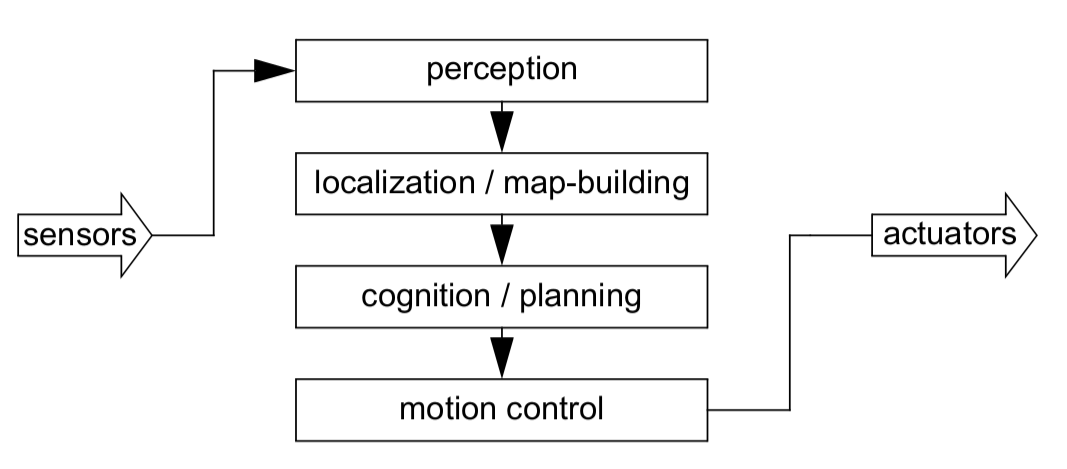
\includegraphics[scale=0.23]{high_level_strategy}
\caption{A common architecture which is employed for map-based navigation. This architecture is comprised of 4 phases: perception, localisation/map building, path planning, and motion control. (Siegwart \& Nourbakhsh, 2004).}
\end{minipage}
\end{figure}

%-------------------------------------------------------------
\section{Map Building}
Complicated tasks such as exploration and object avoidance can be undertaken without an internal representation of the robot's environment, however, some tasks such as absolute localisation or path planning become increasingly difficult to solve. According to Elfes (1989) the most natural representation of a robot's environment is a map. This section of the critical analysis compares the advantages and disadvantages of using a mapping scheme, or not mapping scheme.
\begin{figure}[h]
\centering
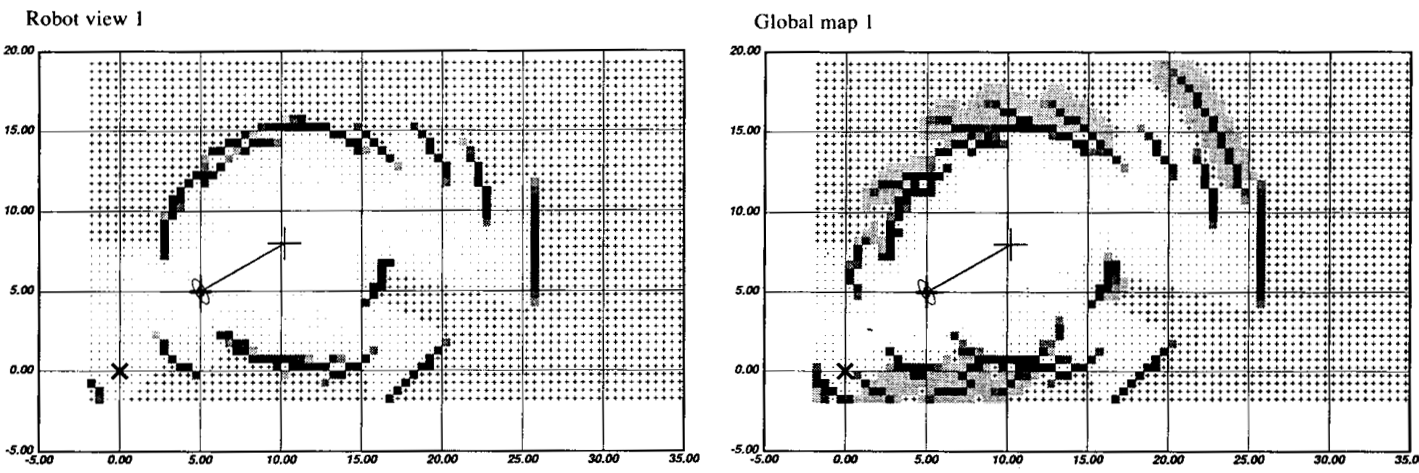
\includegraphics[scale=0.3]{occupancy_grid}
\caption{An example of a mobile robot mapping an unknown environment using an occupancy grid, taken from Alberto Elfes' 1989 paper \textit{Using Occupancy Grids for Mobile Robot Perception and Navigation}}
\end{figure}

One of the single most common approaches to mapping is a fixed decomposition of an environment. This method was famously pioneered by Alberto Elfes in 1989, who referred to this representation as an \textit{occupancy grid}. Elfes builds an \textit{occupancy grid} by overlaying the environment using a set of discrete cells, as shown in Figure 26. Each of the grid's cells is either filled (by part of an obstacle) or is empty (part of free space). \textit{Occupancy grid} mapping is attractive as it allows the user to build a representation of the environment using data from multiple sensors of different type - referred to as sensor fusion in the literature. Given the stochastic nature of the sensor data, Elfes employed a probabilistic approach to determine whether a cell was occupied or not. This method turned out to computationally expensive, and in 1991, Borenstein \& Koren improved on Elfes method for updating cells using a \textit{Vector Field Histogram}.

\begin{figure}[h]
\centering
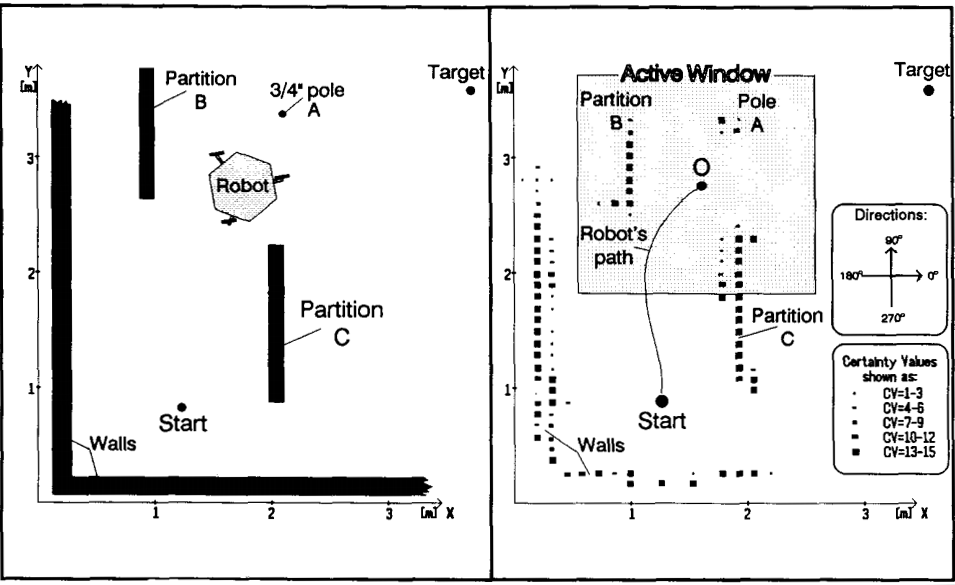
\includegraphics[scale=0.3]{vfh_occ_grid}
\caption{This picture is taken from Borenstein \& Koren's paper titled \textit{The Vector Field Histogram - Fast Obstacle Avoidance for Mobile Robots}. The right hand panel shows the robot's environment, and the left hand panel shows the occupancy grid representation of that environment, which has been built using a \textit{Vector Field Histogram}}
\end{figure}

Essentially, Borenstein \& Koren updated the occupancy of cells in the robot's active window at the sensor sampling frequency. The microprocessor would receive sensor data, and if the sensor detected an obstacle, then the cell value corresponding to the obstacle location was incremented by 1. Simultaneously, every cell value between the detected obstacle, and the robot was decremented by 1. The high frequency update of this approach represented a probability distribution similar to that of a histogram. Cell values were allowed to vary from 0 which represented free space, up to 15 which represented a high certainty that the cell contained an obstacle. Figure 27 shows an example environment on the left, and a corresponding histogram representation on the right. The advantages of Borenstein \& Koren's approach was that it achieved similar results as Elfes' \textit{occupancy grid}, but was significantly less expensive from a computational standpoint. Table 11 provides a summary of the advantages and disadvantages of not mapping an environment compared with mapping an environment.

\begin{table}[h]
\centering
\caption{Summary on the advantages and disadvantages of not mapping, and mapping using a occupancy grid approach}\footnotesize
\begin{tabular}{cp{7.5cm}p{0.1cm}p{7.5cm}}
\toprule
 & \textbf{No Mapping} & & \textbf{Mapping with an Occupancy Grid} \\
\midrule
\multirow{2}{*}[-0.15cm]{\rotatebox[origin=c]{90}{\textbf{Advantages}}} & \begin{itemize}[leftmargin=0.3cm] \item Simple to implement \item Does not require memory \item Computationally fast \end{itemize} & & \begin{itemize}[leftmargin=0.3cm] \item Provides the robot with access to more sophisticated navigation, path planning, and obstacle avoidance strategies \end{itemize} \\
\midrule
\multirow{2}{*}[-0.25cm]{\rotatebox[origin=c]{90}{\textbf{Disadvantages}}} & \begin{itemize}[leftmargin=0.3cm] \item Leaves robot with limited options for navigation strategies, and obstacle avoidance \item The full environment may never be explored since the robot has not internal construct of what it has and has not explored \end{itemize} & & \begin{itemize}[leftmargin=0.3cm] \item There is a memory requirement to store the map \item Higher levels of map fidelity require finer map discretisation resulting in greater memory requirements \item Technically challenging to implement \end{itemize} \\
\bottomrule
\end{tabular}
\end{table}
\newpage

%-------------------------------------------------------------
\section{Absolute Localisation}
\begin{figure}[h]
\begin{minipage}{0.45\textwidth}
Gutmann \& Fox (1998) define localisation as the task of estimating position and orientation of a mobile robot in some environment. Goel, Roumeliotis, \& Sukhatme (1998) provide further distinction using two subcategories: relative localisation and absolute localisation. They define these subcategories as follows:
\begin{itemize}
\item \textbf{Relative localisation:} evaluating the position and orientation using information provided by various on-board sensors, such as optical rotary encoders
\item \textbf{Absolute localisation:} obtaining the absolute position using environmental landmarks, or beacons
\end{itemize}

Why is absolute localisation important? As previously noted, techniques which calculate relative localisation, such as odometry, are imperfect - they are prone to the accumulation of error. This is due to approximations used in dynamic equations governing robot motion, and errors from the sensor readings that odometry depends on. This can lead to the robot's internal position belief to diverge from its actual position over time. Odometry is particularly sensitive to errors in orientation - even small orientation errors can lead to large errors in position belief, as shown in Figure 28. Furthermore, this can corrupt the robot's mapping system which path planning and navigation more difficult. An example of this can be seen in Figures 29 and 30. The left panel shows the exact environment map, indicated with thick dark lines. The desired robot trajectory is shown by the light grey line. 
\end{minipage}
\hspace{1cm}
\begin{minipage}{0.45\textwidth}
\centering
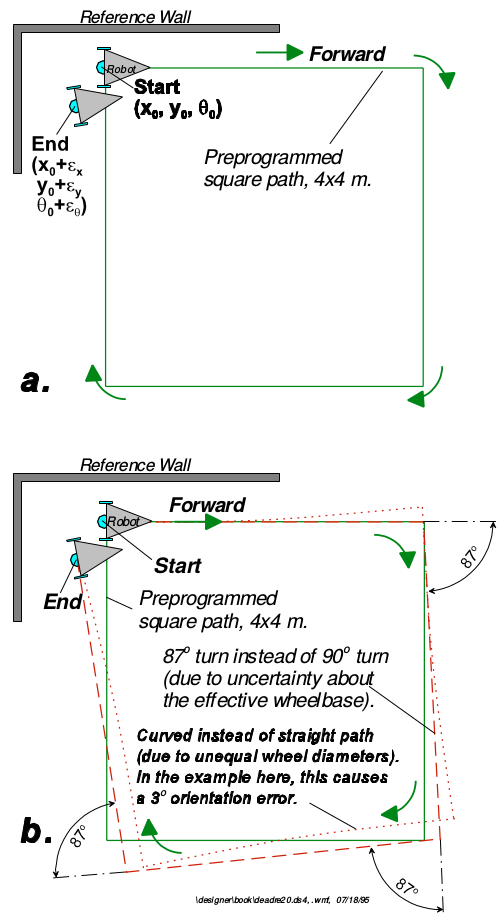
\includegraphics[scale=0.4]{odom_error}
\caption{An example of basic odometry errors taken from Borenstein's book \textit{Where am I now?}}
\end{minipage}
\end{figure}

The middle panel shows the exact robot environment, and the
trajectory which has been corrupted by odometry error. The panel on the right shows the robot’s internalised map
of the environment, which has been corrupted by odometry error. It must be noted that if a robot does not have prior information about the environment, that is the robot is not provided with a map, then an additional problem arises. The robot cannot accurately map if it does not know where it is in the environment, and at the same time the robot cannot know where it truly is if it does not have an accurate map. This problem, in the literature, is known as the simultaneous location and mapping problem (SLAM). According to Durrant-Whyte \& Bailey (2006) the SLAM problem has been solved both theoretically, and for practical implementations. These types of solutions represent state-of-the-art in AWR design, and the implementations of these strategies would take considerable time and cost. The description of how these these methods work are mathematically involved and beyond the scope of this report, however, it must be noted that successful implementation would see increased performance in AWR navigation, obstacle avoidance, and autonomous exploration. Table 12 provides a summary of the advantages and disadvantages associated with having no localisation strategy, and using SLAM.

\begin{figure}[h]
\centering
\begin{minipage}{0.45\textwidth}
\centering
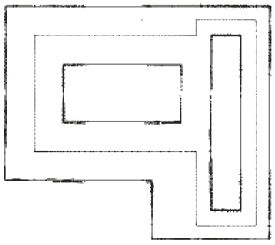
\includegraphics[height=5cm]{exact}
\end{minipage}
\hspace{1cm}
\begin{minipage}{0.45\textwidth}
\centering
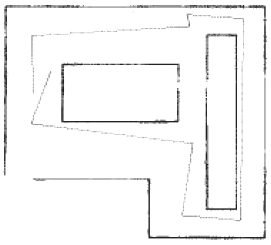
\includegraphics[height=5cm]{exact_odom}
\end{minipage}
\caption{The image on the left shows the exact model of the robot environment (dark line), and the desired trajectory around the environment (light line). The middle image shows the exact robot environment, and the trajectory which has been corrupted by odometry error. Image taken from Okamoto \& Guizilini (2010).}
\end{figure}

\begin{figure}[h]
\centering
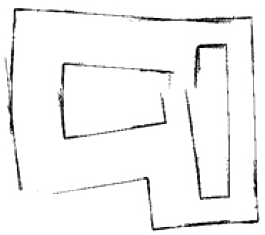
\includegraphics[height=5cm]{odom_error_map}
\caption{Shows the robot's internalised map of the environment, which has been corrupted by odometry error. Image taken from Okamoto \& Guizilini (2010).}
\end{figure}

\begin{table}
\centering
\caption{Summary of the advantages of no absolute localisation implementation, compared to a SLAM impementation}\footnotesize
\begin{tabular}{cp{7cm}p{0.1cm}p{7cm}}
\toprule
 & \textbf{No Localisation} & & \textbf{Simultaneous Localisation \& Mapping (SLAM)}\\
\midrule
\multirow{2}{*}[-0.25cm]{\rotatebox[origin=c]{90}{\textbf{Advantages}}} & \begin{itemize}[leftmargin=0.3cm] \item Easy to implement \item Does not require computational resources \end{itemize} & & \begin{itemize}[leftmargin=0.3cm] \item Provides the robot with the ability to create a map and localise itself within the map, correcting accumulated odometry errors \item Allows precise navigation and map building \end{itemize} \\
\midrule
\multirow{2}{*}[-0.25cm]{\rotatebox[origin=c]{90}{\textbf{Disadvantages}}} & \begin{itemize}[leftmargin=0.3cm] \item Robot accumulates error from using odometric methods of navigation - error may cause incorrect navigation and corrupted mapping  \end{itemize} & & \begin{itemize}[leftmargin=0.3cm] \item Technically challenging to understand \item Technically challenging to implement \item High cost to implement \item Significant use of computational resources \end{itemize} \\
\bottomrule
\end{tabular}
\end{table}

\clearpage
%-------------------------------------------------------------
\section{Exploration Strategy}
Exploration is defined by Yamauchi (1997) as the act of ``moving through an unknown environment". An exploration strategy is implemented in the robot's software, and is a critical design consideration for successful autonomous navigation. This section of the report will look at the advantages and disadvantages of having a basic stochastic exploration strategy, compared to a strategy which is more computationally involved.

\begin{figure}[h]
\begin{minipage}{0.45\textwidth}
A stochastic exploration strategy, sometimes called reactive navigation, implements the AWR with with a set of behaviours which are triggered when the robot encounters some known environmental structure. A simple example of would be software which tells the robot to drive straight until it's sensors locate an obstacle in front of the robot. The detected obstacle would trigger the robot to stop and initiate a 90$^o$ turn to the right (or left). The robot would then continue in a straight line until it reached another obstacle. The strategy is referred to as stochastic because the robot bounces around the environment in a randomised way.
\end{minipage}
\hspace{1cm}
\begin{minipage}{0.45\textwidth}
\centering
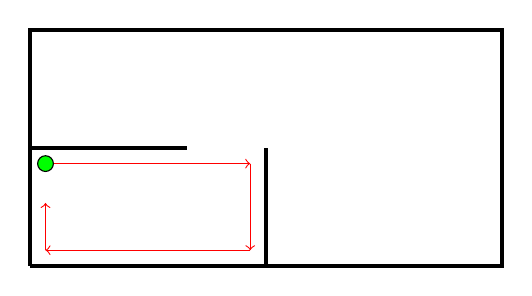
\begin{tikzpicture}
% Drawing environment
\draw[thick, line width=1.5pt] (0,0)--(6,0)--(6,3)--(0,3)--(0,0);
\draw[thick, line width=1.5pt] (3,0)--(3,1.5);
\draw[thick, line width=1.5pt] (0,1.5)--(2,1.5);

% Drawing robot path
\draw[red, ->] (0.2,1.3) -- (2.8,1.3);
\draw[red, ->] (2.8,1.3) -- (2.8,0.2);
\draw[red, ->] (2.8,0.2) -- (0.2,0.2);
\draw[red, ->] (0.2,0.2) -- (0.2,0.8);

% Drawing robot
\draw[fill=green] (0.2,1.3) circle (0.1cm);
\end{tikzpicture}
\caption{A simple example of environment design which would cause a robot with simple stochastic exploration strategy to fail. This figure shows the robot (a green circle) becoming trapped in an environment structure forever.}
\end{minipage}
\end{figure}

A stochastic exploration strategy is desirable because it is simple to implement and only requires minimal computational resources to complete the task. The main disadvantages lie in the fact that the robot may traverse an area of the environment multiple times before it explores all of the environment. Moreover, environmental topologies exist in which the robot could get stuck, referred to as \textit{local minima} in the literature (Siegwart \& Nourbakhsh, 2004). Figure 31 demonstrates the basic exploration strategy described above, and shows an environmental topology in which the robot becomes trapped in a \textit{local minima}. Yamauchi cites the central question to developing a good exploration strategy as:

\vspace{0.5cm}

 \ \ \ \ \textit{Given what you know about the world, where should you move to gain as much new information as possible?}

\vspace{0.5cm}

Yamauchi goes on to posit that an exploration strategy for gaining the most new information is to move the AWR to a boundary between obstacle free open space and uncharted territory. This strategy is referred to as frontier based navigation. The strategy relies on the use of an occupancy grid with additional representation for unexplored cells. At the start of robot navigation each cell is populated with a value, such as -1, indicating that the cell is unknown. When a cell has been explored, using Borenstein and Koren's \textit{Vector Field Histogram} scheme outlined in Section 5, the cell is populated with a value ranging from 0 to 15. If a cell is below a certain threshold value (say 2) then it is considered free space.\\

The exploration strategy employs a process analogous to edge detection to find the boundaries between open space and unknown space - any obstacle free cell adjacent to an uncharted cell is labelled as a frontier edge. Frontier edge cells are grouped into frontier regions, and if the frontier region is big enough the centroid of this region is marked as a location that the robot will explore. An example of this process can be seen in Figure 32, which was taken from Yamauchi's 1997 paper \textit{A Frontier-Based Approach for Autonomous Exploration}. The main advantages of this exploration strategy is that it guarantees full environment exploration, given that all areas of the environment are accessible. The principal drawbacks are that the software implementation is not straight forward, and requires more computational resources meaning that a more expensive microprocessor (like the myRIO) is required. Table 13 provides a summary on the advantages and disadvantages of stochastic exploration and frontier based exploration.

\begin{figure}[h]
\centering
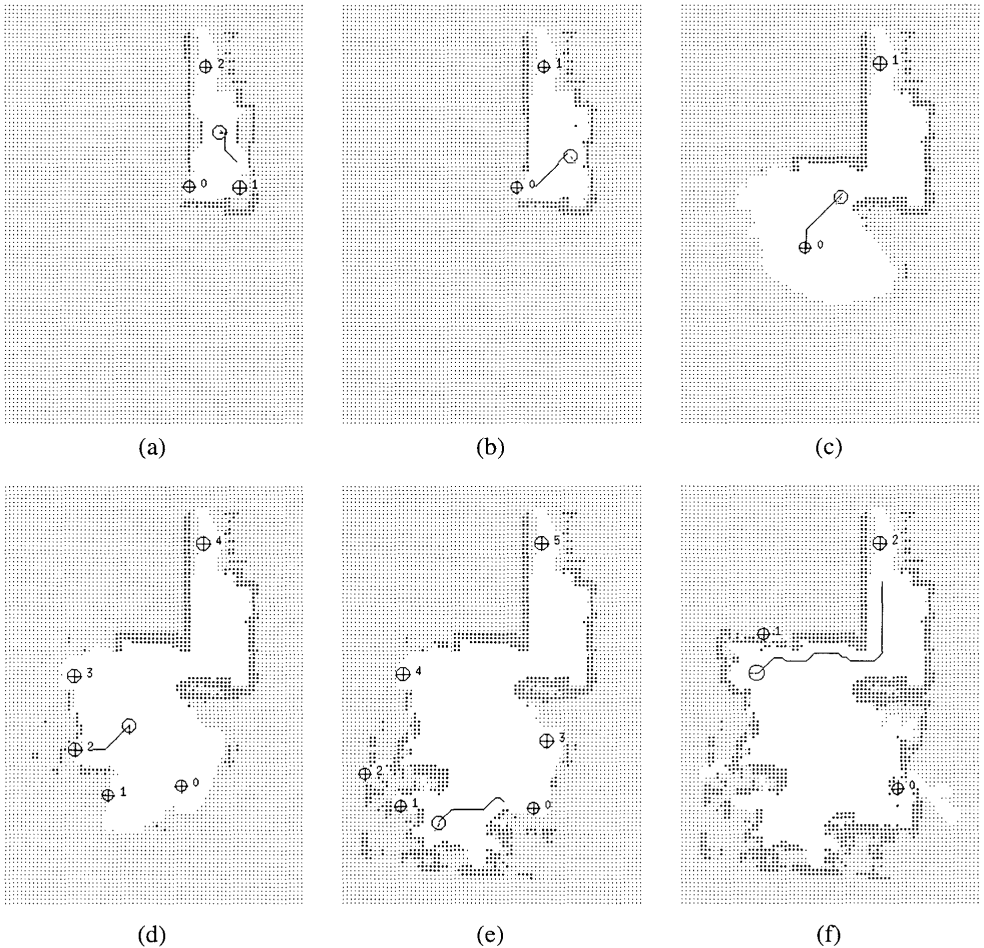
\includegraphics[scale=0.5]{frontier_exploration}
\caption{A picture illustrating Frontier-Based autonomous exploration taken from Yamauchi's 1991 paper titled \textit{A Frontier-Based Approach for Autonomous Exploration}. Panel (a) depicts the AWR identifying 3 frontier regions for exploration, and panel (b) shows the AWR navigating to region 0. }
\end{figure}

\clearpage

\begin{table}[h]
\centering
\caption{Summary on the advantages and disadvantages of using a stochastic exploration strategy, or a frontier-based exploration strategy}\footnotesize
\begin{tabular}{cp{7cm}p{0.1cm}p{7cm}}
\toprule
 & \textbf{Stochastic Exploration Strategy} & & \textbf{Frontier-Based Exploration Strategy}\\
\midrule
\multirow{2}{*}[-0.3cm]{\rotatebox[origin=c]{90}{\textbf{Advantages}}} & \begin{itemize}[leftmargin=0.3cm] \item Simple to implement \item Computationally inexpensive \end{itemize} & & \begin{itemize}[leftmargin=0.3cm] \item Guaranteed to explore entire map, provided all map areas are deemed accessible from grid resolution on robot map \item More likely that robot will converge on exit panel \end{itemize} \\
 & & & \\
\midrule
\multirow{2}{*}[-0.3cm]{\rotatebox[origin=c]{90}{\textbf{Disadvantages}}} & \begin{itemize}[leftmargin=0.3cm] \item May lead to robot getting trapped in local minima \item Does not guarantee that entire map will be explored \item Considerable risk that robot will not converge on exit panel \end{itemize} & & \begin{itemize}[leftmargin=0.3cm] \item Computationally expensive \item Technically challenging to implement \end{itemize} \\
 & & & \\
\bottomrule
\end{tabular}
\end{table}
%-------------

%-----------------------------------------------------
\section{Hardware Environment}
\subsection{Computational Device}
There are two computational devices which are permitted to be used for the AWR:
\begin{itemize}
\item \textbf{Arduino:} 8-bit AVR microcontroller wqith 32KB flash memory, 1024B EEPROM. Low cost, low performance.
\item \textbf{myRio:} Xilinx Z-7010 667 MHz processor, 512MB non-volatile, 256MB DDR3. High cost, high performance.
\end{itemize}
\subsection{Power}
There are three main devices that require a power supply namely, the myRIO, the motor controller to drive the motors and the Kinect device. The robot’s motors are rated at 7.2 V, and the myRIO requires a power supply between 6 and 16 V (14W consumption). The Kinect device requires a 12 V supply. To run all of the devices, some power arrangement is necessary. It must be noted that there are two different voltage levels:
\begin{enumerate}
\item 7.2V to run motors
\item 12V to run myRIO and Kinect devices
\end{enumerate}

Each device requires an individual minimum current value, hence appropriate voltage and current supply requirements are critically important. Table 14 summarises the supply requirements for each device.
\begin{table}[h]
\centering
\caption{Summary of the main power requirements key components of the system.}
\begin{tabular}{lrr}
\toprule
\textbf{Device/Equipment} & \textbf{Voltage ($\si{\volt}$)} & \textbf{Current ($\si{\ampere}$)}\\
\midrule
myRIO & 12.00 & 1.20\\
Kinect & 12.00 & 2.00\\
Motors & 7.2 & $<$2.50\\
\bottomrule
\end{tabular}
\end{table}

On a top of the different power supply requirements, there is another concern for electrical supply design. The problem will possibly arise if one supply is used to supply power to all the devices. Brushed DC motors are notorious for introducing EMI (electro-magnetic interference). This interference/noise from the commutator brushes induces noise into the power line. It can interfere with the sensors, and can possibly damage myRIO by causing voltage dips. The motor draws a very high current at the start-up which can cause ripple voltage at the power input to myRIO device. To eliminate the potential problems with the noise, the decision has been made to use two power supplies i.e 9V battery to power robot’s motors and 12V battery to power both myRIO and Kinect device.
%-----------------------------------------------------
\section{Proposed Design Options}
There were three main design options proposed in the statement of work: Low Complexity (Design Option 1), Moderate Complexity (Design Option 2), and High Complexity (Design Option 3). This section provides a list of the hardware elements and design choices for each design, in addition to providing a brief overview of how each system operates.
\subsection{Design Option 1 (Low Complexity)}
\subsubsection{Hardware \& Design Choices}
\begin{table}[h]
\centering
\caption{Summary of the hardware utilised in design option 1}\footnotesize
\begin{tabular}{p{3.5cm}p{3.8cm}p{3.5cm}p{3.8cm}}
\toprule
\textbf{Hardware} & \textbf{Specification} & \textbf{Design Element} & \textbf{Specification}\\
\midrule
& & &\\
Chassis  & \textit{Rover 5} & Mobility Configuration & \textit{Differential Drive with omnidirectional passive wheel}\\
& & &\\
Proprioceptive Sensors & \textit{Optical rotary encoders} & Locomotion Control & \textit{PID}\\
& & &\\
Exteroceptive Sensors & \textit{IR Ranging} & Mapping & \textit{None}\\
& & & \\
Computational Hardware & \textit{Arduino} & Localisation & \textit{None}\\
& & & \\
 & & Exploration Strategy & \textit{Stochastic}\\
& & & \\
\bottomrule
\end{tabular}
\end{table}

\subsubsection{Operation \& Software Description}
\begin{figure}[h]
\begin{minipage}{0.45\textwidth}
This design is low complexity, easy to be constructed and required the lowest cost compared to other 2 options. It is operated by using a finite state machine and four sensors;  one IR sensor on the front used for checking an obstacle-free path forward, two on the left and right side of the robot to assure the robot will not collide with walls and a final sensor will be employed on rear of the robot chassis used to detect if the robot is currently placed on the red exit panel. There are two types of IR sensor used for the design option 1 which are SHARP GP2D120 for the side of the robot and SHARP GP2Y0A21YKOF for the front of the robot. Operation of the design option 1 is shown in Figure 33. Initially, the robot is placed at the starting point as the stop state. The sensors will check through the robot path if there are no obstacles present in the robot path the robot will moves forward using a constant velocity controlled by PID control. If the sensors detect that the path was blocked the robot will change state to the turn state. 
\end{minipage}
\hspace{1cm}
\begin{minipage}{0.45\textwidth}
\centering
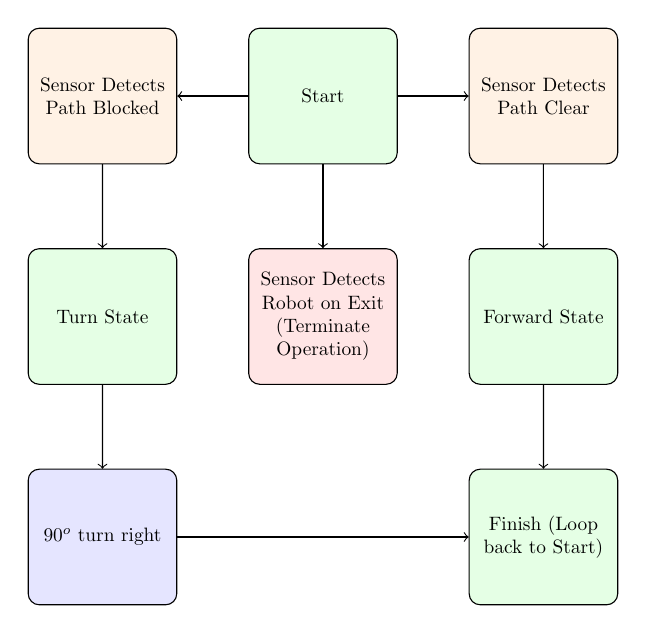
\begin{tikzpicture}[
block/.style={rectangle, draw, minimum width=7em,
text centered, rounded corners, minimum height=7em, text width=7em, fill=green!10, node distance=4cm},
scale=0.7, every node/.style={scale=0.7}
]

\node[block] (start) {Start};
\node[block, left of=start, fill=orange!10] (obsyes) {Sensor Detects Path Blocked};
\node[block, right of=start, fill=orange!10] (obsno) {Sensor Detects Path Clear};
\node[block, below of=start, fill=red!10] (complete) {Sensor Detects Robot on Exit (Terminate Operation)};
\node[block, below of=obsyes] (turn) {Turn State};
\node[block, below of=obsno] (forward) {Forward State};
\node[block, below of=forward] (finish) {Finish (Loop back to Start)};
\node[block, below of=turn, fill=blue!10] (right) {90$^o$ turn right};

\draw[->] (start)--(obsyes);
\draw[->] (start)--(obsno);
\draw[->] (start)--(complete);
\draw[->] (obsyes)--(turn);
\draw[->] (turn)--(right);
\draw[->] (right)--(finish);
\draw[->] (obsno)--(forward);
\draw[->] (forward)--(finish);
\end{tikzpicture}
\caption{Flow diagram demonstrating the basic operation of the software for Design Option 1.}
\end{minipage}
\end{figure}

The robot performs to turn, for left turn the left motor will move forward by 90-degree pivot turn. Similarly, for right turn the right motor will perform reverse by 90-degree turn. Once the robot has completed turning, the robot will automatically transition state back to the stop state. Finally, if the robot’s sensors detect that it is on the red exit panel then the robot will alter state to the finish sate.

\subsection{Design Option 2 (Moderate Complexity)}
\subsubsection{Hardware \& Design Choices}
\begin{table}[h]
\centering
\caption{Summary of the hardware utilised in design option 1}\footnotesize
\begin{tabular}{p{3.5cm}p{3.8cm}p{3.5cm}p{3.8cm}}
\toprule
\textbf{Hardware} & \textbf{Specification} & \textbf{Design Element} & \textbf{Specification}\\
\midrule
& & &\\
Chassis  & \textit{Rover 5} & Mobility Configuration & \textit{Differential Drive with omnidirectional passive wheel}\\
& & &\\
Proprioceptive Sensors & \textit{Optical rotary encoders} & Locomotion Control & \textit{PID}\\
& & &\\
Exteroceptive Sensors & \textit{IR \& Ultrasonic} & Mapping & \textit{Vector Field Histogram}\\
& & & \\
Computational Hardware & \textit{myRio} & Localisation & \textit{None} \\
& & & \\
 & & Exploration Strategy & \textit{Frontier-Based Exploration}\\
& & & \\
\bottomrule
\end{tabular}
\end{table}

\subsubsection{Operation \& Software Description}
Given the nature of the environment where the robot motion is limited to the predetermined terrain boundaries, the localization and mapping can be represented by a grid of uniform cells and the movement of the robotic vehicle is bounded to the valid steps from one cell to another. This way the navigation map can be reduced to the logic matrix with coordinate system. Using the inputs from mapping and the localization, the vehicle path planning algorithm allows robotic vehicle to follow a suitable path to reach the final destination. In line with the project purpose, the logical navigation rules for this design option are to go straight towards the final destination and, in case of obstacles obstructing the way, avoid it. The block diagram of the obstacle detection and path planning is shown below in Figure 34.\\

\begin{figure}[h]
\centering
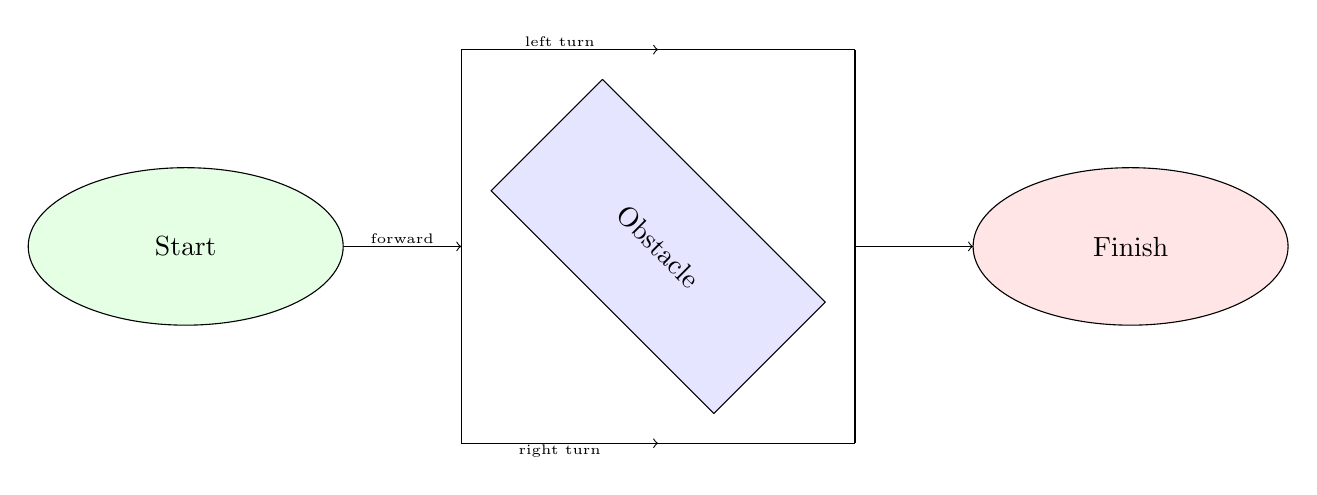
\begin{tikzpicture}
\draw[fill=green!10] (0,0) ellipse (2cm and 1cm);
\draw[shift={(6cm,0cm)},rotate=45,fill=blue!10] (1,2)--(1,-2)--(-1,-2)--(-1,2)--(1,2);
\draw[fill=red!10] (12,0) ellipse (2cm and 1cm);
\node at (0,0) {Start};
\node at (12,0) {Finish};
\node[shift={(6cm,0cm)},rotate=-45] {Obstacle};
\node at (2.75,0.1) {\tiny forward};
\node at (4.75,2.6) {\tiny left turn};
\node at (4.75,-2.6) {\tiny right turn};
\draw[->] (2,0)--(3.5,0);
\draw (3.5,0) -- (3.5,2.5);
\draw (3.5,0) -- (3.5,-2.5);
\draw[->] (3.5,2.5) -- (6,2.5);
\draw[->] (3.5,-2.5) -- (6,-2.5);
\draw (6,2.5)--(8.5,2.5);
\draw (6,-2.5)--(8.5,-2.5);
\draw (8.5,2.5) -- (8.5,0);
\draw (8.5,-2.5) -- (8.5,0);
\draw[->] (8.5,0) -- (10,0);
\end{tikzpicture}
\caption{Navigation strategy for the robotic system.}
\end{figure}

As the robot travels through the environment (grid), it records measurements from its IR and Sonic sensors, the presence of an obstacle inside the angle covered by the sensors sweep area is indicated if the recorded measures from the sensors reach a certain threshold. The robot presence on a place indicates that this place is open to be travelled and empty of obstacles. As the robot travels through the grid it stores the information of the previously visited places as to avoid unnecessarily revisiting locations it has already seen, allowing it to reach the goal faster.\\

\begin{figure}
\begin{minipage}{0.45\textwidth}
The logic diagram of grid exploration can be seen in Figure 35. Firstly the robot checks the surrounding spaces for clearance and moves forward to the next spot, if the robot has finished mapping the maze, it stops its motors. If the robot has not finished mapping the maze, then it will check to see whether there are obstacles in front, to the left, and to the right, which is called a dead end. If the robot identifies itself at a dead end it moves backwards until there is a new spot to check. For instance, if the robot identifies free movement forward and left, the map stores ‘3’, the value for forwards, in position 5 of the array.\\

As the robot continues its travelling through the maze it maps every path in the maze. If the robot identifies itself in a position that was already visited it reorients itself to the next available path from the previous spot. The travelling through the maze continues until the robot reaches its final destination identified by the red square on the terrain. The final destination is detected by the sensor located on the bottom of the robot.
\vspace{0.5cm}
\end{minipage}
\hspace{0.5cm}
\begin{minipage}{0.45\textwidth}
\centering
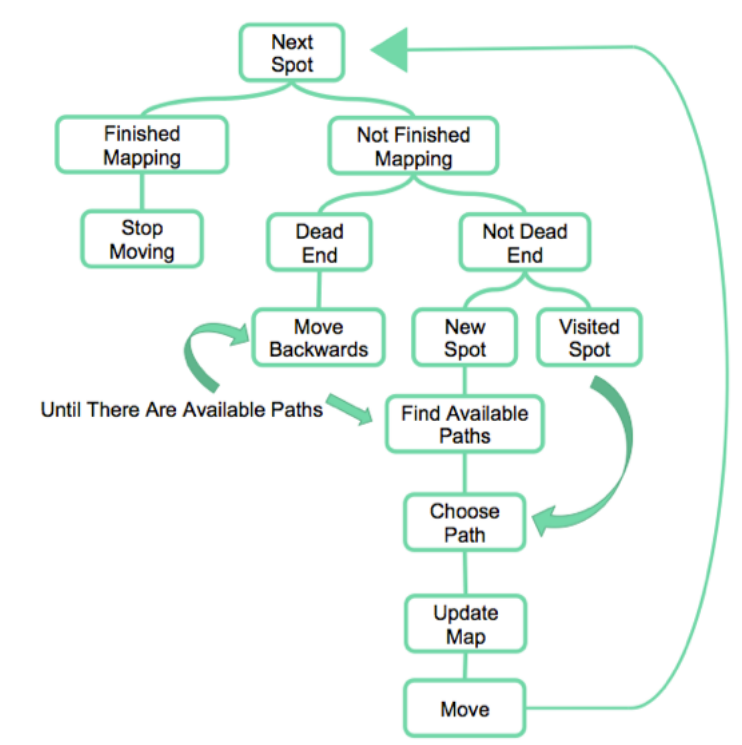
\includegraphics[scale=0.35]{flow_option2}
\caption{The logic diagram for the grid exploration used for Design Option 2.}
\end{minipage}
\end{figure}


\subsection{Design Option 3 (High Complexity)}
\subsubsection{Hardware \& Design Choices}
\begin{table}[h]
\centering
\caption{Summary of the hardware utilised in Design Option 3}\footnotesize
\begin{tabular}{p{3.5cm}p{3.8cm}p{3.5cm}p{3.8cm}}
\toprule
\textbf{Hardware} & \textbf{Specification} & \textbf{Design Element} & \textbf{Specification}\\
\midrule
& & &\\
Chassis  & \textit{Rover 5} & Mobility Configuration & \textit{Differential Drive with omnidirectional passive wheel}\\
& & &\\
Proprioceptive Sensors & \textit{Optical rotary encoders} & Locomotion Control & \textit{PID}\\
& & &\\
Exteroceptive Sensors & \textit{IR, Ultrasonic, \& RGBD} & Mapping & \textit{Vector-Field Histogram}\\
& & & \\
Computational Hardware & \textit{myRio} & Localisation & \textit{SLAM}\\
& & & \\
 & & Exploration Strategy & \textit{Frontier-Based}\\
& & & \\
\bottomrule
\end{tabular}
\end{table}

\subsubsection{Operation \& Software Description}
This design operates in the exact same way as design option 2, however, the Microsoft Kinect that is equipped provides two additional functions:
\begin{itemize}
\item The additional data captured by the Kinect is used in a sensor fusion arrangement with the IR and ultrasonic sensors to provide higher fidelity mapping - more sensors contributing to the \textit{Vector-Field Histogram} map, means the map is more accurate;
\item The Kinect will provide a rich enough dataset to implement an absolute localisation strategy (SLAM), which will be used to correct errors in \textit{odometry}
\end{itemize}

\begin{figure}[h]
\begin{minipage}{0.45\textwidth}
As the robot moves around the map using the Frontier-Based exploration strategy, encoder information is used to predict the measurement of the robot's position, and sensor data is used to create a map of the environment using \textit{Vector-Field Histogram} mapping. The Kinect sensor readings are used to develop a 3D point cloud, which the SLAM algorithm uses determine where the robot is located. The \textit{odometry} position and SLAM estimate position are compared. If the positions match, then the robot continues as normal. If the positions don't match, then the robot checks to see if the the observations are expected, or unexpected. If the observations are expected then the robot will correct the odometry position. If the results are unexpected then the robot will reduce the credibility of the current map, and continue as normal.\\

Figure 35 illustrates the basic operation of the robotic platform, and acts as a high level flow diagram for the implementation of the software.
\end{minipage}
\hspace{0.5cm}
\begin{minipage}{0.45\textwidth}
\centering
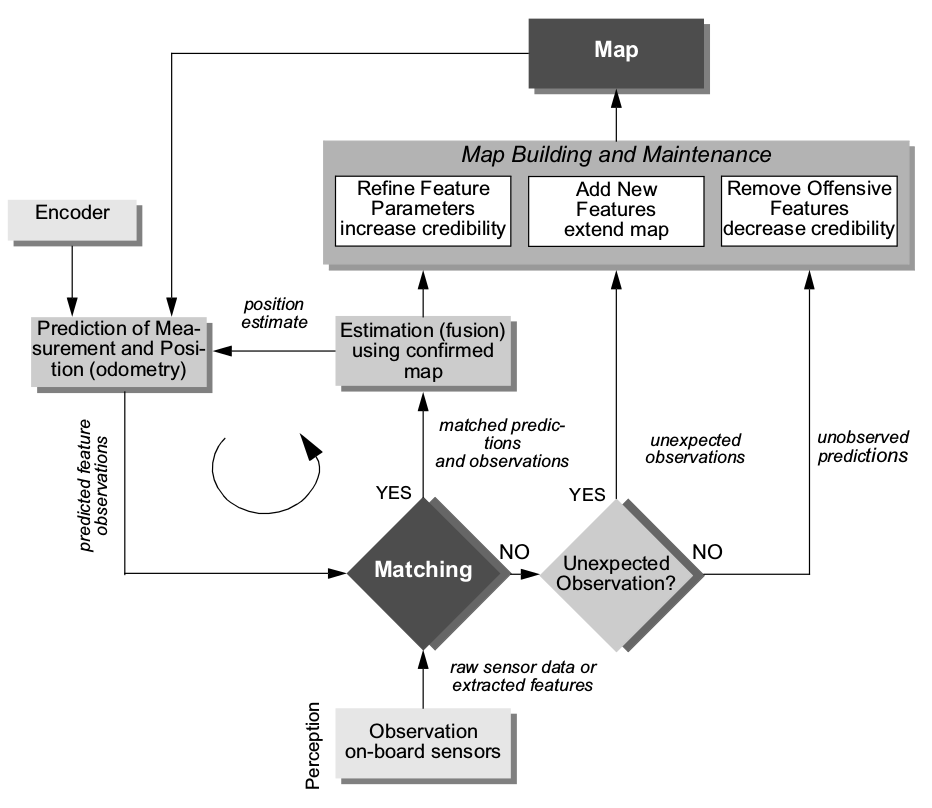
\includegraphics[scale=0.27]{localisation_SLAM}
\caption{Flow diagram demonstrating how SLAM corrects the errors in \textit{odometry} information}
\end{minipage}

\end{figure}

%-----------------------------------------------------
\section{Budgets \& Timeframes}
Each of the three design options require the use of the Rover 5 chassis, the 4 channel motor controller, and the NI myRio Xilinx processor. The main differentiation in terms of cost comes down to the sensors that will be employed and the estimated man hours involved with the implementation. Table 18 provides the estimated budget for each option. The range of costs for the proposed options start at \$1018.56 for the cheapest option, up to \$1464.16 for the state of the art solution. The estimated man hours spent on each of the design options are as follows:\\
\begin{table}[h]
\centering
\caption{Estimated time for each design option}\footnotesize
\begin{tabular}{lr}
\toprule
\textbf{Design Option} & \textbf{Time Spent}\\
\midrule
Design Option 1 & 60 hours\\
Design Option 2 & 100 hours\\
Design Option 3 & 120 hours\\
\bottomrule
\end{tabular}
\end{table}

The costs for these products were sourced from the the following online retailers:
\begin{itemize}
\item \textbf{Mouser:} \url{https://au.mouser.com}
\item \textbf{National Instruments} \url{https://www.ni.com}
\end{itemize}

Project time frame estimations are depicted using a Gantt chart which can be found on page 31.
\begin{table}[h]
\centering
\caption{Budgeted costs for the sunk costs, and each design option}
\begin{tabular}{p{6cm}rp{6cm}r}
\toprule
\textbf{Sunk Costs} & & \textbf{Low Complexity} & \\
\midrule
Rover 5 chassis & \$68.81 & 3 $\times$ SHARP GP2D120 & \$47.85 \\
myRio 1900 & \$814.00 & 1 $\times$ SHARP GP2Y0A21YK0F & \$15.95 \\
4 channel motor controller & \$21.95 &  & \\
Prototyping equipment (breadboard, wiring, etc) & \$50.00 & & \\
\midrule
Total & \$ 954.76 & Total & \$63.80 \\
\midrule
\ & & & \\
\midrule
\textbf{Moderate Complexity} & & \textbf{High Complexity} & \\
\midrule
3 $\times$ SHARP GP2D120 & \$47.85 & 2 $\times$ SHARP GP2D120 & \$32.90 \\
1 $\times$ SHARP GP2Y0A21YK0F & \$15.95 & Intel RealSense R200 Camera & \$127.50 \\
1 $\times$ PING))) Ultrasonic distance sensor & \$29.99 & (optional) Scanse Lidar Sweep Scanner & \$349.00 \\
\midrule
Total & \$93.79 & Total & \$509.40 \\
\bottomrule
\end{tabular}
\end{table}

\newpage

%-----------------------------------------------------
\section{Critical Analysis Evaluation \& Recommended Option}
The evaluation of final design can be broken up into two categories:
\begin{itemize}
\item Elements which do not vary with each of the 3 design options (\textbf{Design Option Invariant Elements}); and
\item Elements which do vary with each of the 3 design options (\textbf{Design Option Variant Elements}) 
\end{itemize}
Every design option has its advantages and disadvantages; hence it’s important to weight each attribute according to how this element performs against the criteria and requirements set by the client. This report uses five main characteristics to assess all design choices - these are outlined as follows:

\begin{itemize}
\item \textbf{Speed (25\% weighting):} one of the main requirement for this design project is speed, the vehicle can operate perfectly and execute the tasks but if it fails to execute it within 3 minutes, the task is deemed as failed. It is one of the most important factors.
\item \textbf{Risk of failure (25\% weighting):} risk of not executing the key milestones that make up the task 
\item \textbf{Time to build (25\% weighting):} the longer it takes to build the product the less time is left for testing and removal of errors.
\item \textbf{Complexity (15\% weighting):} complex design puts at risk the execution of the task due to limited timeframe.
\item \textbf{Cost (10\% weighting):} it’s always least desirable to spend extra budget on the design. For the client the least spending is the best, but the trade-off is the quality. In this design task, the budget is not a main constraint, hence is not as important as the technical factors and functional compliance.
\end{itemize}
\newpage
\subsection{Evaluation of Design Option Invariant Elements}
This section of the report provides an evaluation of those elements of the design which do not vary with each of the design options. Notably, these are the Mobility Configuration, the choice of Proprioceptive Sensors, and the Low Level Control Scheme. The evaluation is undertaken in the table below, with the most desirable design elements highlighted in green. A final design recommendation is provided in Section 11.3.
\vspace{1cm}
\begin{table}[h]
\centering
\footnotesize
\begin{tabular}{|>{\centering\arraybackslash}m{2.5cm}|>{\centering\arraybackslash}m{2cm}|>{\centering\arraybackslash}m{2cm}|>{\centering\arraybackslash}m{2cm}|>{\centering\arraybackslash}m{2cm}|>{\centering\arraybackslash}m{2cm}||>{\centering\arraybackslash}m{2cm}|}
\hline
\rowcolor{gray!95}
\multicolumn{7}{l}{\color{white}\textbf{Mobility Configuration (Section 2)}}\\
\hline
\rowcolor{red!10}
 & 25\% & 25\% & 25\% & 15\% & 10\% & \\
\hline
\rowcolor{gray!10}
\textbf{Design Choice} & \textbf{Speed} & \textbf{Risk of Failure} & \textbf{Time to Build} & \textbf{Complexity} & \textbf{Cost} & \textbf{Score} \\
\hline
Four motors, with Swedish 45 wheels \newline & 90 & 80 & 20 & 20 & 20 & 52.50 \\
\hline
Two motors, with tracked wheels \newline & 60 & 50 & 80 & 80 & 90 & 68.50\\
\hline
\rowcolor{green!10}
Two wheels, with one passive spherical wheel & 80 & 80 & 60 & 70 & 70 & 72.50\\
\rowcolor{gray!95}
\multicolumn{7}{l}{\color{white}\textbf{Proprioceptive Sensor (Section 3.1)}}\\
\hline
\rowcolor{red!10}
 & 25\% & 25\% & 25\% & 15\% & 10\% & \\
\hline
\rowcolor{gray!10}
\textbf{Design Choice} & \textbf{Speed} & \textbf{Risk of Failure} & \textbf{Time to Build} & \textbf{Complexity} & \textbf{Cost} & \textbf{Score} \\
\hline
\rowcolor{green!10}
Optical Rotary Encoders (\textit{Odometry}) & N/A & 70 & 90 & 80 & 90 & 61.00\\
\hline
IMU (\textit{Inertial Navigation}) \newline & N/A & 50 & 60 & 60 & 60 & 42.50\\
\hline
\rowcolor{gray!95}
\multicolumn{7}{l}{\color{white}\textbf{Low Level Locomotion Control (Section 4.1)}}\\
\hline
\rowcolor{red!10}
 & 25\% & 25\% & 25\% & 15\% & 10\% & \\
\hline
\rowcolor{gray!10}
\textbf{Design Choice} & \textbf{Speed} & \textbf{Risk of Failure} & \textbf{Time to Build} & \textbf{Complexity} & \textbf{Cost} & \textbf{Score} \\
\hline
Open Loop Control \newline & N/A & 40 & 70 & 70 & N/A & 38.00 \\
\hline\rowcolor{green!10}
Closed Loop Control (PID) \newline & N/A & 70 & 50 & 60 & N/A & 39.00 \\
\hline
\end{tabular}
\end{table}
\newpage
\subsection{Evaluation of Design Option Variant Elements}
This section of the report provides an evaluation of those elements of the design which vary with each of the design options. Notably, these are the Computational Hardware, Exteroceptive Sensors, Mapping Strategy, Localisation Strategy, and Exploration Strategy. The evaluation is undertaken in two parts. The first table determines a score for each of the design elements, for each of the three design options. The set of scores for each of design options are totalled in the final evaluation seen in subsection 11.3 - the most desirable design option is highlighted in green.
\vspace{1cm}
\begin{table}[h]
\centering
\footnotesize
\begin{tabular}{|>{\centering\arraybackslash}m{2.5cm}|>{\centering\arraybackslash}m{2cm}|>{\centering\arraybackslash}m{2cm}|>{\centering\arraybackslash}m{2cm}|>{\centering\arraybackslash}m{2cm}|>{\centering\arraybackslash}m{2cm}||>{\centering\arraybackslash}m{2cm}|}
\hline
\rowcolor{gray!95}
\multicolumn{7}{l}{\color{white}\textbf{Computational Hardware (Section 8.1)}}\\
\hline
\rowcolor{red!10}
 & 25\% & 25\% & 25\% & 15\% & 10\% & \\
\hline
\rowcolor{gray!10}
\textbf{Design Choice} & \textbf{Speed} & \textbf{Risk of Failure} & \textbf{Time to Build} & \textbf{Complexity} & \textbf{Cost} & \textbf{Score} \\
\hline
Design Option 1 (\textit{Arduino}) & N/A & N/A & 60 & 70 & 70 & 32.50 \\
\hline
Design Option 2 (\textit{myRIO}) & N/A & N/A & 50 & 50 & 30 & 23.00\\
\hline
Design Option 3 (\textit{myRIO}) & N/A & N/A & 50 & 50 & 30 & 23.00\\
\hline
\rowcolor{gray!95}
\multicolumn{7}{l}{\color{white}\textbf{Exteroceptive Sensor (Section 3.2)}}\\
\hline
\rowcolor{red!10}
 & 25\% & 25\% & 25\% & 15\% & 10\% & \\
\hline
\rowcolor{gray!10}
\textbf{Design Choice} & \textbf{Speed} & \textbf{Risk of Failure} & \textbf{Time to Build} & \textbf{Complexity} & \textbf{Cost} & \textbf{Score} \\
\hline
Design Option 1 \tiny(\textit{SHARP IR Ranging}) \newline & N/A & N/A & 60 & 80 & 90 & 36.00\\
\hline
Design Option 2 \tiny(\textit{Fusion of IR and Ultrasonic Ranging}) & N/A & N/A & 50 & 70 & 70 & 30.00\\
\hline
Design Option 3 \tiny(\textit{Fusion of IR, Ultrasonic, \& RGBD camera}) & N/A & N/A & 20 & 30 & 40 & 13.50\\
\hline
\rowcolor{gray!95}
\multicolumn{7}{l}{\color{white}\textbf{Mapping (Section 5)}}\\
\hline
\rowcolor{red!10}
 & 25\% & 25\% & 25\% & 15\% & 10\% & \\
\hline
\rowcolor{gray!10}
\textbf{Design Choice} & \textbf{Speed} & \textbf{Risk of Failure} & \textbf{Time to Build} & \textbf{Complexity} & \textbf{Cost} & \textbf{Score} \\
\hline
Design Option 1 \tiny(\textit{No Mapping}) \newline & 20 & 20 & 90 & 80 & 90 & 53.50\\
\hline
Design Option 2 \tiny(\textit{Vector Field Hist.}) \newline & 80 & 80 & 50 & 50 & 60 & 66.00\\
\hline
Design Option 3 \tiny(\textit{Vector Field Hist.}) \newline & 80 & 80 & 50 & 50 & 60 & 66.00\\
\hline
\rowcolor{gray!95}
\multicolumn{7}{l}{\color{white}\textbf{Localisation (Section 6)}}\\
\hline
\rowcolor{red!10}
 & 25\% & 25\% & 25\% & 15\% & 10\% & \\
\hline
\rowcolor{gray!10}
\textbf{Design Choice} & \textbf{Speed} & \textbf{Risk of Failure} & \textbf{Time to Build} & \textbf{Complexity} & \textbf{Cost} & \textbf{Score} \\
\hline
Design Option 1 (\textit{None}) & N/A & 50 & 90 & 90 & 60 & 54.50\\
\hline
Design Option 2 (\textit{None}) & N/A & 50 & 90 & 90 & 60 & 54.50\\
\hline
Design Option 3 (\textit{None}) & N/A & 90 & 20 & 10 & 40 & 33.00\\
\hline
\rowcolor{gray!95}
\multicolumn{7}{l}{\color{white}\textbf{Exploration Strategy (Section 7)}}\\
\hline
\rowcolor{red!10}
 & 25\% & 25\% & 25\% & 15\% & 10\% & \\
\hline
\rowcolor{gray!10}
\textbf{Design Choice} & \textbf{Speed} & \textbf{Risk of Failure} & \textbf{Time to Build} & \textbf{Complexity} & \textbf{Cost} & \textbf{Score} \\
\hline
Design Option 1 (\textit{Stochastic}) & 10 & 10 & 90 & 80 & 80 & 47.50\\
\hline
Design Option 2 (\textit{Frontier-Based}) & 90 & 80 & 20 & 20 & 20 & 52.50\\
\hline
Design Option 3 (\textit{Frontier-Based}) & 90 & 80 & 20 & 20 & 20 & 52.50\\
\hline
\end{tabular}
\end{table}

\subsection{Final Recommendation} \normalsize
Summarising the findings from Sections 11.1 and 11.2 the final design should utilise two wheels, with one passive omnidirectional spherical wheel for it's mobility configuration. Optical encoders should be used to calculate the \textit{odometry} of the robot, and closed loop control (preferably PID) should be employed for the low level control of the motors. Design Option 2 (Moderate Complexity) is the most desirable design option. This would see final design employ the myRIO as the computational hardware. Further, the design would employ 4 $\times$ IR ranging sensors: 1 $\times$ SHARP GP2D120 at the front of the robot, and 2 $\times$ SHARP GP2Y0A21YKOF at either side of the robot, and 1 $\times$ SHARP GP2Y0A21YKOF mounted underneath the robot to detect the red exit panel. An ultrasonic sensor would also be employed at the front of the robot. The sensor most likely to be utilised is the Matbotix MB1230 ultrasonic sensor. Both IR and ultrasonic sensors would be used in fusion arrangement to provide information to the robot's mapping system which is based on a modified \textit{occupancy grid} called a \textit{Vector-Field Histogram}. The robot would not employ an absolute localisation strategy, however, would use a \textit{Frontier-Based} exploration strategy to identify areas of interest on the map.
\vspace{1cm}
\begin{table}[h]
\centering
\footnotesize
\begin{tabular}{|>{\centering\arraybackslash}m{2.5cm}|>{\centering\arraybackslash}m{2cm}|>{\centering\arraybackslash}m{2cm}|>{\centering\arraybackslash}m{2cm}|>{\centering\arraybackslash}m{2cm}|>{\centering\arraybackslash}m{2cm}||>{\centering\arraybackslash}m{2cm}|}
\hline
\rowcolor{gray!95}
\multicolumn{7}{l}{\color{white}\textbf{Final Evaluation}}\\
\hline
 & \multirow{2}{*}[-0.3cm]{\rotatebox[origin=c]{90}{\textbf{Comp Hardware}}} & \multirow{2}{*}[-0.3cm]{\rotatebox[origin=c]{90}{\textbf{Exteroceptive Sn}}}  & \multirow{2}{*}[-0.3cm]{\rotatebox[origin=c]{90}{\textbf{Mapping}}} & \multirow{2}{*}[-0.3cm]{\rotatebox[origin=c]{90}{\textbf{Localisation}}} & \multirow{2}{*}[-0.3cm]{\rotatebox[origin=c]{90}{\textbf{Exploration Stg}}} & \multirow{2}{*}[-0.3cm]{\rotatebox[origin=c]{90}{\textbf{Total}}} \\

& & & & & & \\
& & & & & & \\
& & & & & & \\
& & & & & & \\
& & & & & & \\
& & & & & & \\
& & & & & & \\
& & & & & & \\
\hline
Design Option 1 & 32.50 & 36.00 & 53.50 & 54.50 & 47.50 & 224.00\\
\hline
\rowcolor{green!10}
Design Option 2 & 23.00 & 30.00 & 66.00 & 54.50 & 52.50 & 226.00 \\
\hline
Design Option 3 & 23.00 & 13.50 & 66.00 & 33.00 & 52.50 & 188.00 \\
\hline
\end{tabular}
\end{table}

\clearpage

\section{References}
\normalsize
Barshan, B., \& Durrant-Whyte, H. (1993). An Inertial Navigation System for a Mobile Robot. \textit{IEEE Conference on Intelligent Robots and Systems}, Yokohama, Japan, July 26-30, 1993.\\

\normalsize
Borenstein, J., Everett, H., \& Feng, L. (1996). Where am I? \textit{University of Michigan for ORNL D\&D program}.\\

\normalsize
Borenstein, J., \& Koren, Y. (1991). Histogramic Mapping for Mobile Robot Obstacle Avoidance. \textit{IEEE Transactions on Robotics and Automation}, 7 (4) pp 535-539.\\

\normalsize
Dudek, G., \& Jenkin, M. (2010). Computational Principals of Mobile Robotics. \textit{Cambridge University Press} [Kindle version]. Retrieved from \url{http://www.amazon.com}.\\

Dudek, G., \& Jenkin, M. (2008). Inertial Sensors, GPS, and Odometry. \textit{Springer Handbook of Robotics}.\\DOI: 10.1007/978-3-540-30301-5\_21\\

\normalsize
Durrant-Whyte, H., \& Bailey, T. (2006). Simultaneous Localization and Mapping: Part 1. \textit{IEEE Robotics \& Automation Magazine}, pp 99-108.\\

\normalsize
Elfes, A. (1989). Using Occupancy Grids for Mobile Robot Perception and Navigation. {IEEE}. Retrieved from \url{https://ieeexplore.ieee.org}\\

\normalsize
Everett, H. (1995). Sensors for Mobile Robots. \textit{AK Peters Ltd}, Massachusetts.\\

\normalsize
Ganganath, N. \& Leung, (2012). Mobile Robot Localisation using Odometry and Kinect Sensor. \textit{2012 IEEE International Conference on Emerging Signal Processing Applications}. DOI: 10.1109/ESPA.2012.6152453\\

\normalsize
Goel, P., Roumeliotis, S., \& Sukhatme, G. (1998). Robot Localisation Using Relative and Absolute Position Estimates. \textit{Department of Computer Science, Institute for Robotics and Intelligent Systems}.\\ 

\normalsize
Gutmann, J., \& Fox, D. (1998). An Experimental Comparison of Localisation Methods Continued. \textit{Department of Computer Science \& Engineering, University of Washington}.\\

\normalsize
Ippoliti, G., Jetto, L., \& Longhi, S. (2005). Localisation of mobile robots: Development and comparative evaluation of algorithms based on odometric and inertial sensors. \textit{Journal of Field Robotics}, 22 (12). \url{https://doi.org/10.1002/rob.20095}\\

\normalsize
Kamarudin, K., Mamduh, S., Shakaff, A., \& Zakaria, A. (2014). Performance Analysis of the Microsoft Kinect Sensor for 2D Simultaneous Localisation and Mapping (SLAM) Techniques. \textit{Open Access Sensors}.\\

\normalsize
Kapoor, S., Mahesh, K., Ruzinov, D., \& Battipaglia, J. (2017). Autonomously Solving Mazes with Robots. Retrieved from \small\url{http://soe.rutgers.edu/sites/default/files/imce/gov2017/AutonomouslySolvingMazeswithRobots.pdf}.\\

\normalsize
Leung, J. (2003). Studies on Map Building and Exploration Strategies for Autonomous Mobile Robots. (Doctoral dissertation). \textit{Hong Kong Polytechnic University}.\\

\normalsize
Ogata, K. (2010). Modern Control Engineering Fifth Edition. \textit{Pearson Education Inc}.\\ 

\normalsize
Okamoto, J., \& Guizilini, V. (2010). On-line SLAM using clustered landmarks with omnidirectional vision. \textit{Journal of Brazilian Society of Mechanical Sciences and Engineering}, Vol 32.\\

\normalsize
Reynolds, S. (2018). 3D Perception Report. \url{https://github.com/skreynolds/RoboND_reports/blob/master/03_perception_3d/03_perception_3d.pdf}\\

\normalsize
Rover 5 Datasheet. (2018). Retrieved from \url{https://www.sparkfun.com/datasheets}.\\

\normalsize
Siegwart, \& R., Nourbakhsh, I. (2004). Autonomous Mobile Robots. \textit{The MIT Press Cambridge, Massachusetts}.\\

\normalsize
Yamauchi, B. (1997). A Frontier-Based Approach for Autonomous Exploration. \textit{Navy Center for Applied Research in Artificial Intelligence}.\\

\begin{sidewaysfigure}[p]
\centering
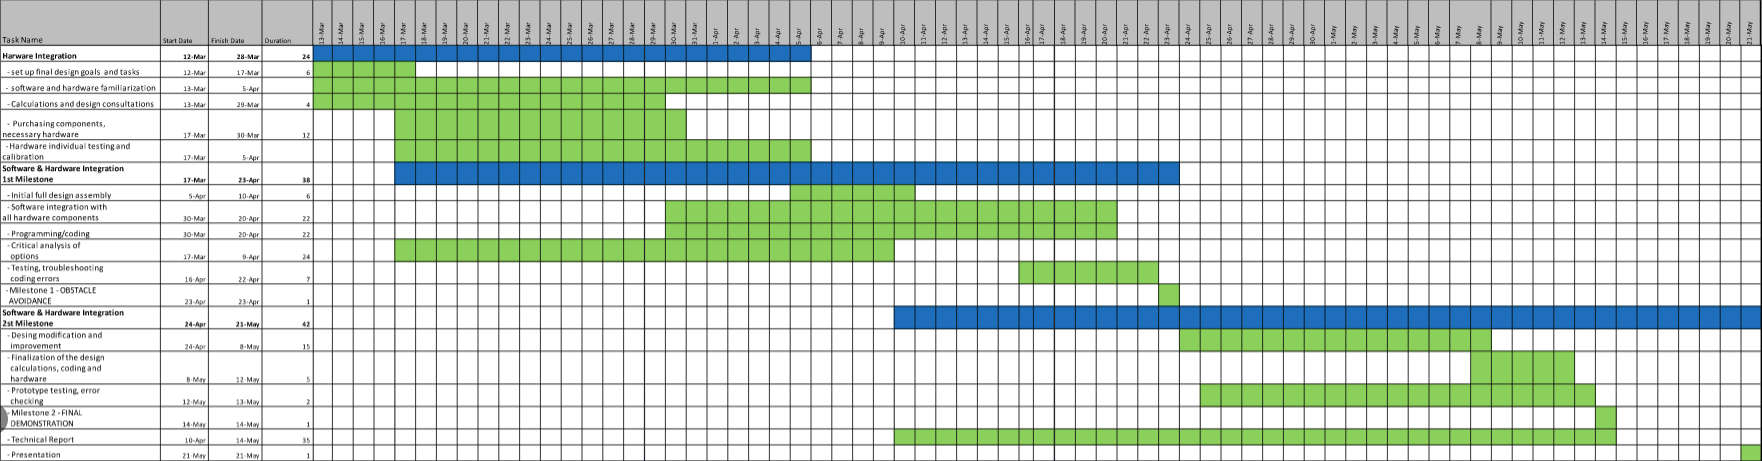
\includegraphics[scale=0.38]{gantt_chart}
\caption{A gantt chart breaking down the phases of the project and detailing the labour assignment through the project life cycle.}
\end{sidewaysfigure}

\end{document}